\documentclass[a4paper]{article}
\usepackage{hcmut}
% Khai báo tcolorbox với tham số [most] để load toàn bộ thư viện nâng cao (đổ bóng, vẽ viền, box title,...)
\usepackage[most]{tcolorbox} 
\usepackage{xcolor}
\usepackage{geometry}
\usepackage{amsmath}
\usepackage{booktabs}
\usepackage{array}
\usepackage{colortbl}
\usepackage{fancyhdr}
\usepackage{titlesec}
\usepackage{enumitem}
\usepackage{hyperref}
\usepackage{float}



\definecolor{lightblue}{RGB}{220,235,250}
\definecolor{rowgray}{RGB}{245,245,245}
% Định nghĩa các màu dùng cho các Style
\definecolor{bkblue}{RGB}{0, 85, 164}    % Dùng cho Cách 1
\definecolor{darkgray}{RGB}{50, 50, 50}  % Dùng cho Cách 3
\begin{document}
\begin{titlepage}
\begin{tikzpicture}[remember picture,overlay,inner sep=0,outer sep=0]
     \draw[blue!70!black,line width=4pt] ([xshift=-1.5cm,yshift=-2cm]current page.north east) coordinate (A)--([xshift=1.5cm,yshift=-2cm]current page.north west) coordinate(B)--([xshift=1.5cm,yshift=2cm]current page.south west) coordinate (C)--([xshift=-1.5cm,yshift=2cm]current page.south east) coordinate(D)--cycle;

     \draw ([yshift=0.5cm,xshift=-0.5cm]A)-- ([yshift=0.5cm,xshift=0.5cm]B)--
     ([yshift=-0.5cm,xshift=0.5cm]B) --([yshift=-0.5cm,xshift=-0.5cm]B)--([yshift=0.5cm,xshift=-0.5cm]C)--([yshift=0.5cm,xshift=0.5cm]C)--([yshift=-0.5cm,xshift=0.5cm]C)-- ([yshift=-0.5cm,xshift=-0.5cm]D)--([yshift=0.5cm,xshift=-0.5cm]D)--([yshift=0.5cm,xshift=0.5cm]D)--([yshift=-0.5cm,xshift=0.5cm]A)--([yshift=-0.5cm,xshift=-0.5cm]A)--([yshift=0.5cm,xshift=-0.5cm]A);

     \draw ([yshift=-0.3cm,xshift=0.3cm]A)-- ([yshift=-0.3cm,xshift=-0.3cm]B)--
     ([yshift=0.3cm,xshift=-0.3cm]B) --([yshift=0.3cm,xshift=0.3cm]B)--([yshift=-0.3cm,xshift=0.3cm]C)--([yshift=-0.3cm,xshift=-0.3cm]C)--([yshift=0.3cm,xshift=-0.3cm]C)-- ([yshift=0.3cm,xshift=0.3cm]D)--([yshift=-0.3cm,xshift=0.3cm]D)--([yshift=-0.3cm,xshift=-0.3cm]D)--([yshift=0.3cm,xshift=-0.3cm]A)--([yshift=0.3cm,xshift=0.3cm]A)--([yshift=-0.3cm,xshift=0.3cm]A);

\end{tikzpicture}
\begin{center}
    \textbf{ĐẠI HỌC QUỐC GIA THÀNH PHỐ HỒ CHÍ MINH}
    \vspace{7pt}
    
    \textbf{TRƯỜNG ĐẠI HỌC BÁCH KHOA}
    
    \vspace{7pt}
    
    \textbf{KHOA KHOA HỌC VÀ KỸ THUẬT MÁY TÍNH}
\end{center}
\begin{center}
 % Kéo logo VNU-HCM sang trái 1.5cm
    \begin{figure}[htbp]
        \centering
        \includegraphics[scale=0.3]{Images/bachkhoa_logo.png}
    \end{figure}
    \vspace{-20pt}
    \fontsize{18pt}{17pt}
    \selectfont
    \textbf{REPORT LAB LOGIC DESIGN}
    \vspace{16pt}
    \hrule
    \vspace{10pt}
    %\textit{\textbf{Đề tài}}\\ [10pt]
    \textcolor{blue}{\Large{\textbf{ASSIGNMENT 2: NETWORK DESIGN AND SIMULATION FOR A CRITICAL LARGE HOSPITAL}}}\\
    \vspace{10pt}
    \hrule
\end{center}

\begin{center}
    \fontsize{16pt}{20pt}\selectfont
    \textbf{GVHD: Bùi Xuân Giang}
\end{center}

\begin{adjustbox}{width=0.8\textwidth,center=\textwidth} % Adjusted width to fit within \textwidth
    \small
        \begin{tabular}{|>{\centering\arraybackslash}m{1cm}|>{\centering\arraybackslash}m{5.5cm}|>{\centering\arraybackslash}m{3cm}|>{\centering\arraybackslash}m{1.55cm}|} % Increased width of "Nhiệm vụ" column
            \hline
            \textbf{STT} & \textbf{Full name} & \textbf{Students ID} & \textbf{Class}\\
            \hline
            1 & Tào Nguyễn Tâm Phúc & 2312716 & L02 \\
            \hline
            2 & Nguyễn Hoàng Minh Phú & 2312655 &  L02 \\
            \hline
            3 & Lê Thanh Phong & 2312618 &  L02 \\
            \hline
            4 & Nguyễn Đình Thịnh & 2313281 & L02 \\
            \hline
            5 & Nguyễn Doãn Quang & 2312794 & L02 \\
            \hline
        \end{tabular}
\end{adjustbox}
\begin{center}
    \vspace{10pt}
    %\textit{Ho Chi Minh City, 12/2025}
\end{center}
\end{titlepage}
\newpage
\tableofcontents
% \input{Sections/1-Title}
\section{PHÂN TÍCH YÊU CẦU HỆ THỐNG VÀ XÁC ĐỊNH CẤU TRÚC MẠNG PHÙ HỢP}

\subsection{Phân tích yêu cầu hệ thống mạng của Trụ sở chính và hai chi nhánh phụ}
Mô hình mạng của Bệnh viện được thiết kế theo kiến trúc phân tán, bao gồm một Trụ sở chính (Main Site) đóng vai trò đầu não và hai Chi nhánh phụ (Auxiliary Sites). Mỗi phân khu mang một đặc thù riêng về chức năng hoạt động và cấu trúc không gian, đòi hỏi một thiết kế mạng đảm bảo tính liên tục, bảo mật nghiêm ngặt và khả năng mở rộng linh hoạt.

\subsubsection{Yêu cầu hạ tầng đối với Trụ sở chính (Main Site)}
\begin{itemize}
    \item \textbf{Cấu trúc không gian:} Trụ sở chính được cấu thành từ hai khối nhà độc lập là Tòa A và Tòa B. Mỗi tòa nhà được xây dựng với quy mô 5 tầng, mỗi tầng bao gồm 10 phòng ban chức năng. Toàn bộ các phòng đều được trang bị hệ thống máy tính, thiết bị y tế chuyên dụng và thiết bị ngoại vi để phục vụ công tác khám chữa bệnh.
    \item \textbf{Khu vực trung tâm kỹ thuật:} Trung tâm dữ liệu (Data Center), phòng IT và phòng điều hành cáp (Cabling Central) được quy hoạch tại một khu vực biệt lập, cách hai tòa nhà chính khoảng 50 mét. Đây là "trái tim" của hệ thống, tập trung toàn bộ hạ tầng cốt lõi bao gồm máy chủ, tường lửa (firewall), Switch Core, Router trung tâm, hệ thống Patch Panel, nguồn điện dự phòng UPS và hệ thống điều hòa kiểm soát môi trường.
    \item \textbf{Quy mô thiết bị và Công nghệ:} Hạ tầng mạng phải đáp ứng kết nối cho khoảng 600 máy trạm, 10 máy chủ trung tâm và ít nhất 12 thiết bị chuyển mạch/định tuyến. Mạng phải hỗ trợ khả năng tích hợp thêm các thiết bị bảo mật chuyên dụng trong tương lai. Về mặt công nghệ, hệ thống sử dụng mạng quang thụ động GPON kết hợp cùng chuẩn GigaEthernet (1/10/40 GbE). Môi trường mạng yêu cầu phủ sóng Wi-Fi toàn diện và áp dụng mô hình phân tách VLAN cho từng khu vực chức năng riêng biệt.
    \item \textbf{Kết nối diện rộng (WAN):} Trụ sở chính kết nối với hai chi nhánh (tại đường DBP và BHTQ) thông qua hai kênh truyền thuê riêng (leased lines). Hệ thống phải tích hợp cơ chế cân bằng tải (load balancing) nhằm tối ưu băng thông và tạo dự phòng chống lỗi. Điểm lưu ý quan trọng là toàn bộ lưu lượng Internet của toàn hệ thống đều phải được định tuyến qua Trụ sở chính.
    \item \textbf{Cơ chế bảo mật và An ninh:} Hạ tầng sử dụng kết hợp giữa phần mềm bản quyền và mã nguồn mở. Các lớp phòng thủ bao gồm Tường lửa (Firewall), hệ thống phát hiện và ngăn chặn xâm nhập (IDS/IPS), cùng các chính sách chống tấn công Phishing. Mạng được chia tách rõ ràng giữa vùng phi quân sự (DMZ) và mạng người dùng nội bộ. Đồng thời, hệ thống Camera giám sát IP được phủ rộng toàn bệnh viện, kết hợp cùng VPN Site-to-Site và VPN Teleworker để mã hóa luồng dữ liệu.
\end{itemize}

\subsubsection{Yêu cầu hạ tầng đối với Chi nhánh phụ (Auxiliary Sites)}
\begin{itemize}
    \item \textbf{Cấu trúc không gian:} Mỗi chi nhánh phụ có quy mô gồm 2 tầng hoạt động. Phòng IT và phòng Cáp trung tâm được thiết kế đặt tại tầng 1 để thuận tiện cho việc kéo cáp và quản lý.
    \item \textbf{Quy mô thiết bị:} Mỗi cơ sở phụ tải mạng cho khoảng 260 máy trạm, 2 máy chủ cục bộ và tối thiểu 5 thiết bị mạng. Toàn bộ dữ liệu của chi nhánh được kết nối đồng bộ về Trụ sở chính thông qua hệ thống WAN.
\end{itemize}

\subsubsection{Các tiêu chuẩn chung về hiệu năng}
\begin{itemize}
    \item \textbf{Đặc tính lưu lượng:} Mạng phải chịu tải được 80\% tổng lưu lượng phát sinh trong ngày dồn vào các khung giờ cao điểm (từ 9h-11h sáng và 15h-16h chiều).
    \item \textbf{Khả năng mở rộng:} Hạ tầng thiết kế phải dự trù khả năng tăng trưởng 20\% về quy mô người dùng và băng thông trong vòng 5 năm tới. Bắt buộc duy trì tính sẵn sàng cao (High Availability) và khả năng khắc phục thảm họa (Disaster Recovery) nhanh chóng.
    \item \textbf{Thông số ước tính lưu lượng:} 
    \begin{itemize}
        \item Hệ thống máy chủ: Tải xuống (Download) 1000 MB/ngày, Tải lên (Upload) 2000 MB/ngày.
        \item Máy trạm (Workstations): Tải xuống 500 MB/ngày, Tải lên 100 MB/ngày.
        \item Thiết bị khách truy cập Wi-Fi: Tải xuống trung bình 500 MB/ngày.
    \end{itemize}
\end{itemize}

\subsection{Đánh giá và Khảo sát thực tế}
Việc khảo sát thực địa tại Trụ sở chính và hai chi nhánh phụ là bước bắt buộc để thu thập thông số môi trường triển khai. Các hạng mục khảo sát được tóm tắt trong bảng sau:


\begin{longtable}{|c|>{\raggedright\arraybackslash}p{4cm}|>{\raggedright\arraybackslash}p{9cm}|}
\hline
\textbf{STT} & \textbf{Hạng mục khảo sát} & \textbf{Nội dung chính cần kiểm tra / ghi chú} \\ \hline

% Xóa bỏ hoàn toàn phần \endfirsthead và \endhead ở đây

1 & Thông tin chung & Người liên hệ tại site (tên, chức vụ, SĐT), sơ đồ mặt bằng, lịch triển khai, khu vực khảo sát cụ thể. \\ \hline
2 & Thiết bị và điểm kết nối (Endpoints) & Số lượng máy trạm, thiết bị y tế, camera, Access Point hiện hữu, thiết bị sử dụng Wi-Fi khách. \\ \hline
3 & Cơ sở hạ tầng vật lý & Phòng IT / Data Center, tủ rack, patch panel, cáp mạng hiện có, hệ thống điện UPS. \\ \hline
4 & Cáp mạng và cáp quang & Loại cáp (Cat6, Fiber), số lượng sợi, đường đi giữa các tòa / tầng, khoảng cách ước tính, tình trạng thực tế. \\ \hline
5 & Khảo sát Wi-Fi & Vị trí dự kiến đặt Access Point, vật cản (tường, thiết bị), khu vực cần phủ sóng mạnh (ICU, sảnh, phòng khám). \\ \hline
6 & Mạng WAN / Internet & Đầu vào ISP, số lượng đường truyền, nhà cung cấp, loại kết nối (MPLS / Internet), thiết bị biên. \\ \hline
7 & Bảo mật và quản trị & Camera, kiểm soát truy cập phòng IT, lưu trữ dữ liệu, xác thực người dùng, sao lưu cấu hình. \\ \hline
8 & Điện và an toàn & Nguồn điện, UPS dự phòng, tiếp địa (grounding), nhiệt độ - độ ẩm, hệ thống báo cháy. \\ \hline
9 & Ứng dụng và dịch vụ & Hệ thống HIS, PACS, mail, VoIP, dịch vụ cloud; yêu cầu backup, DR hoặc kết nối đặc biệt. \\ \hline
10 & Ghi chú thêm & Chi phí dự kiến, hạn chế thương hiệu, yêu cầu hỗ trợ từ IT nội bộ, điều kiện thi công, kho chứa thiết bị. \\ \hline
\end{longtable}

\subsection{Định vị các khu vực có tải trọng mạng cao (Bottleneck Areas)}
Căn cứ vào mô hình luân chuyển dữ liệu, các vùng sau đây được đánh giá là phải chịu áp lực xử lý đặc biệt lớn:
\begin{itemize}
    \item \textbf{Phòng trung tâm kỹ thuật (Cách 50m tại Main Site):} Khu vực này là nơi đặt toàn bộ máy chủ và Tường lửa (ASA) của Trụ sở chính. Khối lượng dữ liệu cực lớn đến từ hai tòa A và B, cộng với việc mọi gói tin trao đổi ra Internet đều phải đi qua Tường lửa ASA, khiến đây trở thành điểm tập trung tải trọng lớn nhất của toàn hệ thống.
    \item \textbf{Hệ thống Multilayer Switch tại từng tòa nhà:} Tại mỗi tòa nhà (Tòa A và Tòa B), Multilayer Switch đóng vai trò là xương sống tiếp nhận lưu lượng từ các Access Switch của toàn bộ các tầng. Việc liên tục định tuyến khối lượng dữ liệu từ hàng trăm thiết bị y tế và người dùng tạo ra một mức tải vô cùng lớn.
    \item \textbf{Hệ thống Multilayer Switch tại các chi nhánh:} Tương tự như Trụ sở chính, các Switch đa lớp tại chi nhánh không chỉ tổng hợp dữ liệu nội bộ liên tầng mà còn đảm nhận việc duy trì luồng giao tiếp liên tục với Trụ sở chính thông qua mạng WAN.
\end{itemize}

\indent Do đó, việc tối ưu hóa thiết kế, lựa chọn năng lực thiết bị phần cứng mạnh mẽ và áp dụng các thuật toán cân bằng tải tại các khu vực này là ưu tiên hàng đầu.

\subsection{Mô hình kiến trúc mạng đề xuất}
Hệ thống được thiết kế theo \textbf{Cấu trúc mạng hình sao (Star Topology)} kết hợp với \textbf{Mô hình 3 lớp (Three-tier Network Architecture)}.
\begin{itemize}
    \item \textbf{Ưu điểm của mô hình Hình sao:} Trong kiến trúc này, các nút mạng biên (Access layer) hoạt động hoàn toàn độc lập. Sự cố xảy ra tại một nút mạng sẽ được cô lập, không gây ảnh hưởng đến toàn bộ hệ thống (ngoại trừ lỗi phần cứng tại thiết bị trung tâm). Hệ thống này rất phù hợp với quy mô y tế do chịu tải nặng tốt và dễ dàng bổ sung thiết bị mới.
    \item \textbf{Mô hình 3 lớp (Core, Distribution, Access):} Switch Core Layer 3 tại trung tâm chịu trách nhiệm cao nhất trong việc định tuyến và luân chuyển gói tin tốc độ cao giữa các VLAN.
\end{itemize}
\begin{figure}[H]
    \centering
    % Điều chỉnh [width=0.9\textwidth] để ảnh chiếm 90% chiều rộng trang giấy
    % Thay "ten_anh_cua_ban.png" bằng tên file ảnh thực tế của bạn
    
\includegraphics[width=0.8\textwidth]{images/three-tier.png}
    
    % Tiêu đề của ảnh (giống với caption trong báo cáo mẫu)
    \caption{Mô hình kiến trúc mạng 3 lớp (Three-tier Network Architecture).}
    
    % Nhãn để trích dẫn ảnh trong bài (Ví dụ: "Như được thể hiện trong Hình \ref{fig:three_tier}")
    \label{fig:three_tier}
\end{figure}
\subsection{Thiết kế sử dụng mạng trong môi trường không dây, áp dụng tiêu chuẩn bảo mật và phân vùng hệ thống}

\subsubsection{Tích hợp hệ thống Không dây (Wireless Integration)}
\begin{itemize}
    \item \textbf{Công nghệ Wi-Fi:} Triển khai hàng loạt Access Point (AP) chuẩn Wi-Fi 6. Mô hình \textit{Wireless Mesh} được áp dụng với việc tính toán vị trí AP chiến lược (hành lang, phòng khám, phòng lab) nhằm triệt tiêu vùng lõm sóng (dead zones), đảm bảo băng thông cao và độ trễ thấp.
    \item \textbf{Phân mảnh mạng không dây:} Mỗi khu vực phát hai dải mạng SSID tách biệt:
    \begin{itemize}
        \item \textit{Staff Wi-Fi (VLAN 4):} Mạng nội bộ cho y bác sĩ, yêu cầu mã hóa WPA3 và xác thực người dùng tập trung.
        \item \textit{Guest Wi-Fi (VLAN 5):} Mạng phục vụ bệnh nhân và khách vãng lai, được cô lập hoàn toàn với dữ liệu nội bộ và chỉ cho phép truy cập Internet.
    \end{itemize}
\end{itemize}

\subsubsection{Phân vùng mạng VLAN và Quy hoạch dải IP}
Hệ thống mạng được chia cắt thành các VLAN chuyên biệt dựa trên chức năng nghiệp vụ để giới hạn miền broadcast và tăng tính bảo mật. Trunking được cấu hình trên các cổng Uplink để điều phối nhiều subnet trên một cáp vật lý.
\renewcommand{\arraystretch}{1.3} % Tăng khoảng cách giữa các hàng cho thoáng
\begin{longtable}{|c|l|>{\raggedright\arraybackslash}p{9.5cm}|}
% 1. Phần xuất hiện ở dòng đầu tiên của bảng (Trang đầu)
\hline
\textbf{VLAN ID} & \textbf{Tên VLAN} & \textbf{Mô tả chức năng} \\ \hline
\endfirsthead

% 2. Phần tiêu đề lặp lại ở các trang sau (Để trống theo yêu cầu của bạn)
\endhead

% 3. Phần chân bảng ở các trang bị ngắt (Kẻ đường chỉ ngang)
\hline
\endfoot

% 4. Phần chân bảng ở trang cuối cùng (Chứa đường kẻ ngang và Caption)
\hline
\caption{Bảng phân chia VLAN theo chức năng trong hệ thống mạng bệnh viện}
\label{tab:vlan_chuc_nang} \\
\endlastfoot

% 5. Nội dung dữ liệu của bảng
2 & MEDICAL & Thiết bị y tế, máy móc phòng khám. \\ \hline
3 & LABORATORY & Hệ thống xét nghiệm (LIS). \\ \hline
4 & STAFF WIFI & Phục vụ truy cập không dây cho nhân viên y tế. \\ \hline
5 & GUEST WIFI & Phục vụ truy cập không dây cho bệnh nhân và khách vãng lai. \\ \hline
6 & STORAGE & Quản lý kho bãi và trang thiết bị vật tư. \\ \hline
7 & PHARMACY & Quản lý hệ thống dược phẩm. \\ \hline
8 & CCTV IOT & Kết nối cho hệ thống Camera an ninh và các cảm biến. \\ \hline
9 & HOSPITALSOFTWARE & Dành cho hệ thống lưu trữ/truy xuất hình ảnh y khoa (PACS và RIS). \\ \hline
10 & OFFICE & Dành cho khối hành chính, nhân sự, ban giám đốc. \\ \hline
11 & MANAGEMENT & VLAN cô lập chỉ dành cho quản trị viên và cấu hình thiết bị mạng. \\
\end{longtable}

\subsubsection{Thiết lập vùng phi quân sự DMZ}
Vùng DMZ được thiết lập để đặt các máy chủ cung cấp dịch vụ ra Internet (Web Server, Mail, VPN Gateway, FTP). Đây là vùng đệm cách ly: người dùng Internet có thể truy cập DMZ nhưng không thể từ DMZ xâm nhập ngược vào mạng nội bộ, giúp bảo vệ tài nguyên bệnh viện khi có rủi ro tấn công.

\subsubsection{Giao thức đồng bộ VTP (VLAN Trunking Protocol)}
Distribution Switch sẽ đóng vai trò như một VTP Server, quản lý và đồng bộ hóa thông tin VLAN xuyên suốt hệ thống Access Switch. Kết hợp với DHCP Server, địa chỉ IP được cấp phát tự động cho các máy trạm (Client) một cách đồng nhất, giúp loại bỏ các lỗi do cấu hình thủ công.

\subsubsection{Giao thức định tuyến động OSPF}
Hệ thống sử dụng OSPF (Open Shortest Path First) trong cùng một Area 0 (vùng xương sống - backbone) để kết nối các Router của Trụ sở và Chi nhánh. OSPF trao đổi các gói tin LSA, áp dụng thuật toán Dijkstra để liên tục cập nhật và tìm ra con đường ngắn nhất. Giải pháp này tối ưu băng thông, tự động phục hồi kết nối khi đứt cáp và hỗ trợ quy hoạch mạng hiệu quả (VLSM).

\subsubsection{Thiết lập mạng riêng ảo (VPN Site-to-Site IPsec)}
Để đảm bảo kênh truyền thông bảo mật qua hạ tầng Internet thay vì phụ thuộc hoàn toàn vào kênh WAN, hệ thống triển khai VPN IPsec.
\begin{itemize}
    \item \textbf{Giai đoạn 1 (Phase 1):} Trao đổi khóa và xác thực thông qua Pre-shared Key (ISAKMP SA).
    \item \textbf{Giai đoạn 2 (Phase 2):} Mã hóa luồng dữ liệu bằng chuẩn AES và kiểm tra toàn vẹn bằng thuật toán HMAC-SHA. Chỉ những lưu lượng hợp lệ (dựa trên cấu hình ACL, ví dụ VLAN Management) mới được mã hóa và chui qua hầm VPN (VPN Tunnel).
\end{itemize}

\subsubsection{Triển khai hệ thống Tường lửa (Firewall ASA)}
Cisco ASA Firewall được triển khai làm chốt chặn kiểm soát lưu lượng giữa mạng Inside (Nội bộ), DMZ và Outside (Internet). 
\begin{itemize}
    \item \textbf{Luồng dữ liệu:} Mặc định chỉ cho phép lưu lượng đi từ vùng bảo mật cao (Inside) ra vùng bảo mật thấp (Outside/DMZ). Luồng ngược lại phải tuân thủ nghiêm ngặt các quy tắc ACL.
    \item \textbf{NAT (Network Address Translation):} Dải IP nội bộ và DMZ (ví dụ 10.0.10.0/24) được ẩn danh thông qua NAT động khi truy cập ra Internet.
    \item Tường lửa hoạt động theo nguyên tắc đặc quyền tối thiểu (Least Privilege), đảm bảo an toàn tuyệt đối cho cơ sở dữ liệu y tế.
\end{itemize}
\subsubsection{Hệ thống mạng ngoài và CloudPT}
Các router tại Site chính và hai Site phụ đều tham gia định tuyến OSPF với hệ
thống mạng ngoài. Thành phần CloudPT đóng vai trò mô phỏng hạ tầng Internet,
giúp kiểm thử kết nối WAN thực tế giữa các site.\\
\indent Hệ thống này được giữ lại nhằm thể hiện khả năng mở rộng, bảo mật, và hoạt động
của toàn bộ mô hình mạng khi triển khai thực tế trong môi trường bệnh viện.

\section{Danh sách thiết bị tối thiểu, sơ đồ IP và sơ đồ đi dây}
\subsection{Danh sách các thiết bị tối thiểu}
Theo yêu cầu của dự án thực tế, Bệnh viện cần hạ tầng mạng GigaEthernet 1GbE / 10GbE/ 40GbE. Tuy nhiên, do giới hạn về thư viện thiết bị phần cứng của phần mềm mô phỏng Cisco Packet Tracer, nhóm chúng em quyết định sử dụng các thiết bị có sẵn trong thư viện giả lập (như Router 1941, Switch 3650, Switch 2960) để thiết lập mô hình. Mục đích chính là chứng minh tính đúng đắn của logic mạng, định tuyến, phân chia VLAN và các chính sách bảo mật ACL. Khi triển khai thực tế, các thiết bị này sẽ được thay thế bằng các dòng Enterprise hiện đại tương đương.
\subsubsection{Router}
Router Cisco ISR 2911: Đóng vai trò là Router biên (Edge Router) tại Trụ sở chính và các chi nhánh, chịu trách nhiệm kết nối mạng nội bộ của bệnh viện ra Internet và hệ thống mạng WAN.\\
\indent Thực hiện định tuyến động (OSPF) trên toàn mạng, thiết lập cân bằng tải (Load Balancing), cấu hình NAT, và thiết lập các kênh truyền ảo (VPN Site-to-Site bằng IPsec) để bảo mật dữ liệu y tế giữa các cơ sở.

\begin{tcolorbox}[
        enhanced,
        colback=white,
        colframe=darkgray,
        coltitle=black,
        fonttitle=\large\bfseries,
        title=Thông số kỹ thuật Router Cisco ISR 2911,
        attach boxed title to top left={xshift=5mm, yshift=-3mm},
        boxed title style={colback=white, colframe=darkgray},
        drop fuzzy shadow,
        top=4mm, bottom=2mm, left=2mm, right=2mm
    ]
        \begin{itemize}
            \item \textbf{Cổng kết nối mạng (Tích hợp):} 3 cổng Gigabit Ethernet (10/100/1000 Mbps).
            \item \textbf{Khe cắm mở rộng:} Hỗ trợ các khe cắm module EHWIC/HWIC (dùng để cắm thêm module cổng quang hoặc Serial kết nối Leased Line/MPLS).
            \item \textbf{Bộ nhớ DRAM:} 512 MB (mặc định) / Tối đa 2.5 GB.
            \item \textbf{Bộ nhớ Flash:} 256 MB (mặc định) / Tối đa 8 GB.
            \item \textbf{Tính năng nổi bật:} Hỗ trợ tăng tốc mã hóa phần cứng cho VPN, QoS nâng cao và tích hợp các tính năng bảo mật (Threat Control).
        \end{itemize}
    \end{tcolorbox}

\subsubsection{Access Point}
Access Point AP-PT: Được triển khai làm điểm truy cập không dây chủ đạo trong
toàn bộ mạng bệnh viện. Thiết bị này đảm bảo khả năng kết nối ổn định cho các thiết
bị di động, máy tính xách tay, máy trạm và các thiết bị IoT y tế tại các khu vực như
phòng khám, hành lang, khu chẩn đoán hình ảnh và khu hành chính.\\
\indent AP-PT hoạt động trên băng tần 2.4GHz, cung cấp vùng phủ sóng rộng, đảm bảo
khả năng roaming liền mạch giữa các khu vực. Tín hiệu từ các thiết bị đầu cuối được
truyền đến switch truy cập, từ đó kết nối đến hệ thống mạng lõi. Việc triển khai mạng
Wi-Fi này giúp nhân viên y tế truy cập nhanh chóng vào hồ sơ bệnh án điện tử (EHR)
và hỗ trợ truyền tải dữ liệu theo thời gian thực.
\begin{tcolorbox}[
    enhanced,
    colback=white,
    colframe=darkgray,
    coltitle=black,
    fonttitle=\large\bfseries,
    title=Thông số kỹ thuật Access Point AP-PT,
    attach boxed title to top left={xshift=5mm, yshift=-3mm},
    boxed title style={colback=white, colframe=darkgray},
    drop fuzzy shadow,
    top=4mm, bottom=2mm, left=2mm, right=2mm
]
    \begin{itemize}
        \item \textbf{Cổng kết nối:} Fast Ethernet
        \item \textbf{Băng tần hoạt động:} 2.4GHz
        \item \textbf{Chuẩn Wi-Fi hỗ trợ:} IEEE 802.11 b/g/n
    \end{itemize}
\end{tcolorbox}

\subsubsection{Firewall}
Cisco ASA 5506-X : Được sử dụng làm Firewall tại Trụ sở chính để bảo vệ mạng nội bộ khỏi các mối đe dọa từ Internet.\\
\indent Hỗ trợ tạo nhiều vùng bảo mật khác nhau như Internal, DMZ, External giúp kiểm soát chặt chẽ luồng dữ liệu ra vào. Tích hợp các tính năng tường lửa thế hệ mới (NGFW) và hỗ trợ VPN bảo mật.

\begin{tcolorbox}[
        enhanced,
        colback=white,
        colframe=darkgray,
        coltitle=black,
        fonttitle=\large\bfseries,
        title=Thông số kỹ thuật Cisco ASA 5506-X,
        attach boxed title to top left={xshift=5mm, yshift=-3mm},
        boxed title style={colback=white, colframe=darkgray},
        drop fuzzy shadow,
        top=4mm, bottom=2mm, left=2mm, right=2mm
    ]
        \begin{itemize}
            \item \textbf{Số cổng kết nối:} 8 cổng Gigabit Ethernet[cite: 3].
            \item \textbf{VLAN hỗ trợ:} Tối đa 3 VLAN[cite: 3].
            \item \textbf{Hỗ trợ VPN:} SSL VPN và IPsec VPN[cite: 3].
            \item \textbf{Giao diện quản lý:} ASDM đồ họa[cite: 3].
            \item \textbf{Tính năng bảo mật:} Lọc gói tin, bảo vệ chống DDoS, kiểm soát truy cập ứng dụng[cite: 3].
        \end{itemize}
    \end{tcolorbox}

\subsubsection{Access Switch}
Switch Cisco Catalyst 2960: Được sử dụng làm Switch truy cập (Access Switch) đặt tại các tầng (ví dụ: thiết bị \texttt{Acc-A-F1} tại Tầng 1 - Tòa A).\\
\indent Thiết bị này giúp truyền tải dữ liệu nhanh chóng giữa các khu vực chức năng như
tiếp nhận bệnh nhân, phòng chẩn đoán, khu xét nghiệm và hành chính, đảm bảo hiệu
suất và độ tin cậy cao.

\begin{tcolorbox}[
    enhanced,
    colback=white,
    colframe=darkgray,
    coltitle=black,
    fonttitle=\large\bfseries,
    title=Thông số kỹ thuật Cisco WS-C2960-24TT-L,
    attach boxed title to top left={xshift=5mm, yshift=-3mm},
    boxed title style={colback=white, colframe=darkgray},
    drop fuzzy shadow, % Hiệu ứng đổ bóng mờ
    top=4mm, bottom=2mm, left=2mm, right=2mm
]
    \begin{itemize}
        \item \textbf{Cổng Ethernet:} 24 cổng 10/100 Mbps
        \item \textbf{Cổng uplink Gigabit:} 2 cổng 10/100/1000 Mbps
        \item \textbf{Bộ nhớ DRAM:} 64 MB
        \item \textbf{Bộ nhớ Flash:} 32 MB
    \end{itemize}
\end{tcolorbox}

\subsubsection{Distribution Switch}
Distribution Switch Cisco Catalyst 3650-24PS-L: Dùng làm Switch phân phối, kết nối các Access Switch từ các tầng và khu vực để truyền dữ liệu lên mạng lõi (Core).\\
\indent Thực hiện định tuyến nội bộ giữa các VLAN (Inter-VLAN Routing), quản lý VTP, cung cấp nguồn PoE+ cho các thiết bị tầng dưới, và là điểm hội tụ băng thông.

\begin{tcolorbox}[
        enhanced,
        colback=white,
        colframe=darkgray,
        coltitle=black,
        fonttitle=\large\bfseries,
        title=Thông số kỹ thuật Cisco Catalyst 3650-24PS-L,
        attach boxed title to top left={xshift=5mm, yshift=-3mm},
        boxed title style={colback=white, colframe=darkgray},
        drop fuzzy shadow,
        top=4mm, bottom=2mm, left=2mm, right=2mm
    ]
        \begin{itemize}
            \item \textbf{Cổng Ethernet:} 24 cổng 10/100/1000 Mbps (hỗ trợ PoE+)[cite: 3].
            \item \textbf{Cổng Uplink:} 4 cổng 1G SFP (dùng để cắm cáp quang)[cite: 3].
            \item \textbf{Công suất PoE khả dụng:} 390 W[cite: 3].
            \item \textbf{Dung lượng chuyển mạch:} 88 Gbps[cite: 3].
            \item \textbf{Hiệu suất chuyển tiếp:} 41,66 Mpps[cite: 3].
            \item \textbf{Bộ nhớ:} DRAM 4 GB, Flash 2 GB[cite: 3].
        \end{itemize}
    \end{tcolorbox}
\subsubsection{Server}
Server-PT:Cung cấp các dịch vụ cốt lõi cho hoạt động của Bệnh viện (như quản lý bệnh án HIS, lưu trữ hình ảnh y tế PACS, cơ sở dữ liệu) và các dịch vụ mạng (Web, DNS, DHCP
\begin{tcolorbox}[
        enhanced,
        colback=white,
        colframe=darkgray,
        coltitle=black,
        fonttitle=\large\bfseries,
        title=Thông số kỹ thuật đề xuất cho Server (Thực tế),
        attach boxed title to top left={xshift=5mm, yshift=-3mm},
        boxed title style={colback=white, colframe=darkgray},
        drop fuzzy shadow,
        top=4mm, bottom=2mm, left=2mm, right=2mm
    ]
        \begin{itemize}
            \item \textbf{Lưu ý:} Trong Packet Tracer, nhóm sử dụng \texttt{Server-PT} làm thiết bị mô phỏng chung. Khi triển khai thực tế, Bệnh viện cần trang bị các dòng máy chủ Enterprise mạnh mẽ (ví dụ: Dell PowerEdge R740 hoặc HPE ProLiant DL380 Gen10).
            \item \textbf{Thông số cấu hình dự kiến (Tham khảo):}
            \begin{itemize}
                \item CPU: 2x Intel Xeon Scalable Processors.
                \item RAM: Tối thiểu 128 GB (Có thể mở rộng lên hàng TB cho Database).
                \item Storage: Cấu hình RAID 10 với các ổ cứng SSD NVMe tốc độ cao.
                \item Card mạng (NIC): 2x hoặc 4x cổng 10GbE / 40GbE.
            \end{itemize}
        \end{itemize}
    \end{tcolorbox}

\subsubsection{End Device}
Ngoài các thiết bị trên còn có một số thiết bị khác như: máy chủ, webcam, PC, IoT, ...  

\subsection{Sơ đồ IP}
Hệ thống mạng của bệnh viện sử dụng dải IP Private lớp A (\texttt{10.0.0.0/8}) và được quy hoạch theo mô hình phân cấp (Hierarchical IP Addressing). Cấu trúc IP được thiết kế theo cú pháp \textbf{\texttt{10.[Site].[VLAN].0}}, giúp tối ưu hóa bảng định tuyến OSPF và dễ dàng quản lý các chính sách bảo mật ACL. 

Bên cạnh đó, hệ thống áp dụng kỹ thuật chia mạng con VLSM (Variable Length Subnet Mask) để đáp ứng linh hoạt số lượng thiết bị thực tế, điển hình như việc sử dụng subnet \texttt{/22} cho VLAN Medical tại Trụ sở chính nhằm cung cấp đủ IP cho hơn 600 máy trạm.

\subsubsection{Quy hoạch IP tại Trụ sở chính - Main Site (HCMC)}
Dải mạng phân bổ cho Main Site: \textbf{10.10.0.0/16}

{
    \small % Thu nhỏ chữ một chút để bảng đẹp hơn
    \renewcommand{\arraystretch}{1.3}
    \begin{longtable}{|c|>{\raggedright\arraybackslash}p{6cm}|l|l|}
        \caption{Quy hoạch địa chỉ IP và VLAN tại Trụ sở chính (Main Site)}
        \label{tab:ip_main} \\
        \hline
        \textbf{VLAN} & \textbf{Chức năng (Phân vùng)} & \textbf{Địa chỉ mạng} & \textbf{Subnet Mask} \\
        \hline
        \endfirsthead
        
        \endhead

        \endfoot

        \hline
        \endlastfoot

        10 & Vùng phi quân sự (DMZ) & 10.10.10.0/24 & 255.255.255.0 \\
        \hline
        20 & Server Farm & 10.10.20.0/24 & 255.255.255.0 \\
        \hline
        30 & Management (Quản trị IT) & 10.10.30.0/24 & 255.255.255.0 \\
        \hline
        40 & Medical (Khu vực Y tế - 600+ hosts) & 10.10.40.0/22 & 255.255.252.0 \\
        \hline
        50 & Admin (Hành chính) & 10.10.50.0/24 & 255.255.255.0 \\
        \hline
        60 & Finance (Tài chính - Kế toán) & 10.10.60.0/24 & 255.255.255.0 \\
        \hline
        70 & IT-Ops (Vận hành IT) & 10.10.70.0/24 & 255.255.255.0 \\
        \hline
        80 & HR (Nhân sự) & 10.10.80.0/24 & 255.255.255.0 \\
        \hline
        90 & Camera (Hệ thống giám sát CCTV) & 10.10.90.0/24 & 255.255.255.0 \\
        \hline
        100 & VoIP (Hệ thống điện thoại IP) & 10.10.100.0/24 & 255.255.255.0 \\
        \hline
        110 & Guest Wi-Fi (Mạng Khách) & 10.10.110.0/23 & 255.255.254.0 \\
    \end{longtable}
}
\subsubsection{Quy hoạch IP tại các Chi nhánh phụ (Auxiliary Sites)}
Dải mạng phân bổ cho Chi nhánh DBP: \textbf{10.20.0.0/16} \\
Dải mạng phân bổ cho Chi nhánh BHTQ: \textbf{10.30.0.0/16} \\
\textit{(Do hai chi nhánh có cấu trúc tương đương nhau, quy hoạch VLAN được đồng bộ hóa để thuận tiện cho việc quản lý tập trung).}

{
    \small
    \renewcommand{\arraystretch}{1.3}
    \begin{longtable}{|c|>{\raggedright\arraybackslash}p{6cm}|l|l|}
        \caption{Quy hoạch địa chỉ IP tại các Chi nhánh (Quy ước: X=20 cho DBP, X=30 cho BHTQ)}
        \label{tab:ip_aux} \\
        \hline
        \textbf{VLAN} & \textbf{Chức năng (Phân vùng)} & \textbf{Địa chỉ mạng} & \textbf{Subnet Mask} \\
        \hline
        \endfirsthead
        
        \endhead

        \endfoot

        \hline
        \endlastfoot

        30 & Management & 10.X.30.0/24 & 255.255.255.0 \\
        \hline
        40 & Medical (Khu vực Y tế) & 10.X.40.0/23 & 255.255.254.0 \\
        \hline
        50 & Admin (Hành chính) & 10.X.50.0/24 & 255.255.255.0 \\
        \hline
        60 & Finance (Tài chính - Kế toán) & 10.X.60.0/24 & 255.255.255.0 \\
        \hline
        70 & IT-Ops (Vận hành IT) & 10.X.70.0/24 & 255.255.255.0 \\
        \hline
        80 & HR (Nhân sự) & 10.X.80.0/24 & 255.255.255.0 \\
        \hline
        90 & Camera (Hệ thống giám sát CCTV) & 10.X.90.0/24 & 255.255.255.0 \\
        \hline
        100 & VoIP (Hệ thống điện thoại IP) & 10.X.100.0/24 & 255.255.255.0 \\
        \hline
        110 & Guest Wi-Fi (Mạng Khách) & 10.X.110.0/24 & 255.255.255.0 \\
    \end{longtable}
}

% Thêm lệnh này để ngắt sang trang mới cho sạch sẽ, không bị dính chùm với phần trên


\subsection{Quy hoạch đi dây (Wiring Plan)}

Để đảm bảo hiệu năng, tính dự phòng và khả năng mở rộng cho hệ thống mạng bệnh viện, nhóm áp dụng quy hoạch đấu nối cáp theo cấu trúc phân cấp. Thay vì biểu diễn bằng hình ảnh mạng tổng thể (được trình bày chi tiết ở Bước 4), phần này quy định các chuẩn cáp và tốc độ kết nối vật lý giữa các phân lớp thiết bị trong toàn bộ hệ thống.

% Sử dụng longtable để bảng tự động chia trang mà vẫn đúng thứ tự
{
    \small
    \renewcommand{\arraystretch}{1.4}
    \begin{longtable}{|p{4.5cm}|p{3.5cm}|c|>{\raggedright\arraybackslash}p{6cm}|}
        \caption{Bảng quy chuẩn đấu nối cáp (Wiring Standards) cho hệ thống mạng}
        \label{tab:wiring_plan} \\
        \hline
        \textbf{Kết nối (Từ $\leftrightarrow$ Đến)} & \textbf{Loại cáp} & \textbf{Cổng} & \textbf{Băng thông / Ghi chú} \\
        \hline
        \endfirsthead
        
        \endhead

        \endfoot

        \hline
        \endlastfoot

        Router $\leftrightarrow$ Firewall ASA & Cáp đồng (UTP Cat6) & RJ45 & 1 Gbps (Định tuyến luồng dữ liệu bảo mật) \\
        \hline
        Firewall $\leftrightarrow$ Cụm Server (DMZ) & Cáp quang / Cat6a & SFP/RJ45 & 1 Gbps (Đảm bảo tốc độ truy xuất máy chủ) \\
        \hline
        Core/Dist Switch $\leftrightarrow$ Phân hệ Routing & Cáp quang (Fiber) & SFP & 1 Gbps (Liên kết Uplink tốc độ cao) \\
        \hline
        Distribution $\leftrightarrow$ Access Switch & Cáp quang (Fiber) & SFP & 1 Gbps (Đường Trunking truyền tải đa VLAN) \\
        \hline
        Access Switch $\leftrightarrow$ PC / Laptop & Cáp đồng (UTP Cat6) & RJ45 & 100/1000 Mbps (Kết nối thiết bị đầu cuối) \\
        \hline
        Access Switch $\leftrightarrow$ Access Point & Cáp đồng (UTP Cat6) & RJ45 & 1000 Mbps (Hỗ trợ PoE cấp nguồn cho AP) \\
        \hline
        Access Switch $\leftrightarrow$ Webcam/IoT & Cáp đồng (UTP Cat5e) & RJ45 & 100 Mbps (Cấp nguồn PoE cho thiết bị giám sát) \\
    \end{longtable}
}

\subsubsection{Kiến trúc tổng thể toàn hệ thống (High-level Topology)}

Sơ đồ tổng thể thể hiện cách hệ thống mạng của bệnh viện tương tác với môi trường Internet bên ngoài và sự phân bổ các khu vực trọng yếu. Toàn bộ lưu lượng ra/vào mạng nội bộ đều được kiểm soát bởi cụm Gateway Router và Tường lửa (Firewall ASA).

\begin{figure}[H]
    \centering
    % Nhớ đổi tên file ảnh cho đúng với file của mày
    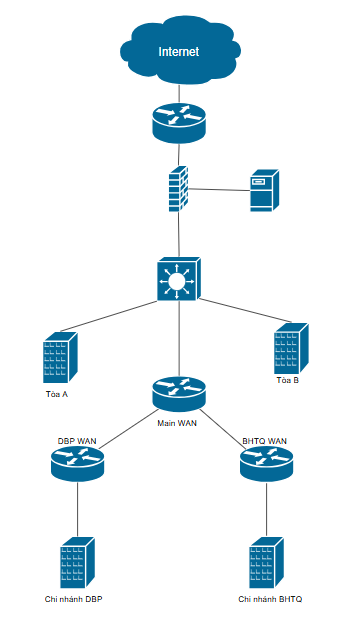
\includegraphics[width=0.5\textwidth]{Images/fullwireplan.png}
    \caption{Sơ đồ kiến trúc mạng logic tổng thể toàn hệ thống}
    \label{fig:logical_tongthe}
\end{figure}

\subsubsection{Sơ đồ chi tiết cụm Trụ sở chính (Main Site)}

Tại Trụ sở chính (HCMC), mạng được thiết kế theo mô hình Core - Distribution - Access. Switch Core (Multilayer Switch 3650) đóng vai trò trung tâm điều phối toàn bộ lưu lượng. Đặc biệt, khu vực Data Center được tách biệt hoàn toàn: vùng DMZ (đặt Web/DNS Server) cắm trực tiếp vào Tường lửa để phục vụ truy cập ngoài, trong khi Server Farm (chứa máy chủ HIS, Database nội bộ) được bảo vệ phía sau Switch Core.

\begin{figure}[H]
    \centering
    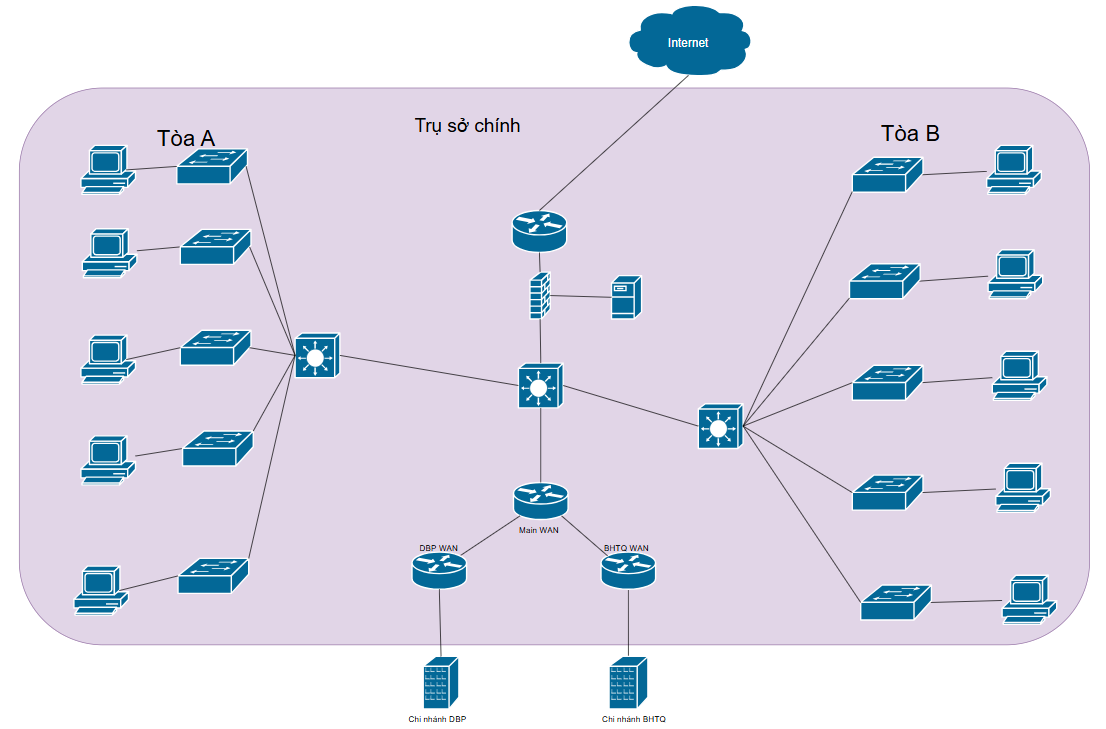
\includegraphics[width=0.95\textwidth]{Images/Maincenter.png}
    \caption{Sơ đồ chi tiết phân vùng hạ tầng mạng tại Trụ sở chính}
    \label{fig:logical_mainsite}
\end{figure}

\subsubsection{Sơ đồ chi tiết kết nối các Chi nhánh (Auxiliary Sites)}

Để đảm bảo kết nối liên tục từ Trụ sở chính đến hai chi nhánh DBP và BHTQ, nhóm sử dụng hạ tầng kết nối WAN (Wide Area Network). Các Router biên (WAN Edge Router) tại Trụ sở chính thiết lập kênh truyền tốc độ cao đến các Router đầu cuối đặt tại mỗi chi nhánh, từ đó phân phối tín hiệu xuống các Core-Switch chi nhánh.

\begin{figure}[H]
    \centering
    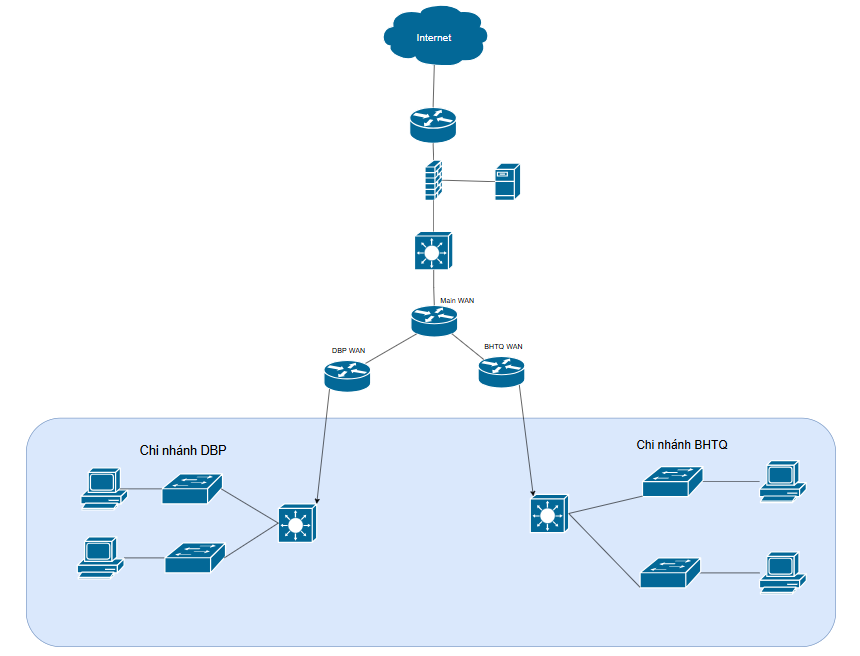
\includegraphics[width=0.95\textwidth]{Images/Chinhanh.png}
    \caption{Sơ đồ chi tiết hạ tầng mạng LAN và kết nối WAN tại các Chi nhánh phụ}
    \label{fig:logical_chinhanh}
\end{figure}
\setcounter{section}{2}
\section{Tính toán thông lượng yêu cầu và băng thông cần thuê từ ISP}

\subsection{Giả định và dữ liệu đầu vào}

Dựa theo đề bài, ta dùng các giả định sau (ghi rõ để dễ kiểm toán):
\begin{itemize}[leftmargin=*, itemsep=2pt]
  \item \textbf{Main Site:} 600 workstation. Mỗi workstation: $\mathrm{DL} = 500$\,MB/day, $\mathrm{UL} = 100$\,MB/day.
  \item \textbf{Servers (tổng toàn hệ):} $\mathrm{DL_{srv}} = 1{,}000$\,MB/day, $\mathrm{UL_{srv}} = 2{,}000$\,MB/day.
  \item \textbf{Wi-Fi khách} (mỗi site): $\mathrm{DL_{wifi}} = 500$\,MB/day.
  \item \textbf{Mỗi Auxiliary Site (DBP, BHTQ):} 260 workstation và Wi-Fi khách 500\,MB/day.
  \item \textbf{Giờ cao điểm:} 80\% tổng lưu lượng tập trung vào 9:00--11:00 (2\,h) và 15:00--16:00 (1\,h) $\Rightarrow$ tổng \textbf{3 giờ peak} mỗi ngày.
  \item Hệ hoạt động 24 giờ/ngày ($86{,}400$\,giây). Quy ước: $1\,\text{MB} = 8\,\text{Mbits}$; kết quả biểu diễn bằng \textbf{Mbps}.
  \item \textbf{Dự phòng tăng trưởng:} $+20\%$ cho 5 năm sau.
\end{itemize}

\subsection{Tính tổng lưu lượng (MB/day)}
Chi tiết phân bổ lưu lượng cho từng phân vùng mạng được tính toán như sau:

\vspace{0.2cm}
\noindent \textbf{1. Trụ sở chính (Main Site)}
\vspace{-0.4cm}
\begin{align*}
  \mathrm{DL_{ws}} &= 600 \times 500 = 300{,}000\ \text{MB/day}, \quad \mathrm{UL_{ws}} = 600 \times 100 = 60{,}000\ \text{MB/day} \\
  \mathrm{DL_{srv}} &= 1{,}000\ \text{MB/day}, \quad \mathrm{UL_{srv}} = 2{,}000\ \text{MB/day}, \quad \mathrm{DL_{wifi}} = 500\ \text{MB/day} \\
  \Rightarrow\quad \mathrm{DL_{main}} &= 300{,}000 + 1{,}000 + 500 = \mathbf{301{,}500}\ \text{MB/day} \\
  \mathrm{UL_{main}} &= 60{,}000 + 2{,}000 = \mathbf{62{,}000}\ \text{MB/day}
\end{align*}

\vspace{0.2cm}
\noindent \textbf{2. Mỗi Auxiliary Site}
\vspace{-0.4cm}
\begin{align*}
  \mathrm{DL_{aux}} &= 260 \times 500 + 500 = \mathbf{130{,}500}\ \text{MB/day} \\
  \mathrm{UL_{aux}} &= 260 \times 100 = \mathbf{26{,}000}\ \text{MB/day}
\end{align*}

\vspace{0.2cm}
\noindent \textbf{3. Hai Auxiliary Site cộng lại}
\vspace{-0.4cm}
\begin{align*}
  \mathrm{DL_{2aux}} &= 2 \times 130{,}500 = 261{,}000\ \text{MB/day} \\
  \mathrm{UL_{2aux}} &= 2 \times 26{,}000 = 52{,}000\ \text{MB/day}
\end{align*}

\vspace{0.2cm}
\noindent \textbf{4. Tổng toàn hệ thống}
\vspace{-0.4cm}
\begin{align*}
  \mathrm{DL_{total}} &= 301{,}500 + 261{,}000 = \mathbf{562{,}500}\ \text{MB/day} \\
  \mathrm{UL_{total}} &= 62{,}000 + 52{,}000 = \mathbf{114{,}000}\ \text{MB/day}
\end{align*}

\subsection{Chuyển đổi sang băng thông (Mbps)}
Áp dụng công thức quy đổi từ dung lượng (MB/day) sang băng thông đường truyền (Mbps):

\vspace{0.2cm}
\noindent \textbf{1. Băng thông trung bình} \\
Công thức: $\displaystyle\text{Mbps} = \dfrac{\text{MB/day} \times 8}{86{,}400}$
\vspace{-0.4cm}
\begin{align*}
  \mathrm{DL_{avg}} &= \frac{562{,}500 \times 8}{86{,}400} \approx \mathbf{52.08\ \text{Mbps}}, \quad
  \mathrm{UL_{avg}} = \frac{114{,}000 \times 8}{86{,}400} \approx \mathbf{10.56\ \text{Mbps}}
\end{align*}

\vspace{0.2cm}
\noindent \textbf{2. Băng thông giờ cao điểm (80\% tổng lưu lượng dồn trong 3 giờ)} \\
Công thức: $\displaystyle\text{Peak (Mbps)} = \dfrac{0.8 \times \text{MB/day} \times 8}{3 \times 3{,}600}$
\vspace{-0.4cm}
\begin{align*}
  \mathrm{Peak\ DL} &= \frac{0.8 \times 562{,}500 \times 8}{10{,}800} \approx \mathbf{333.33\ \text{Mbps}} \\
  \mathrm{Peak\ UL} &= \frac{0.8 \times 114{,}000 \times 8}{10{,}800} \approx \mathbf{67.56\ \text{Mbps}}
\end{align*}

\subsection{Dự phòng tăng trưởng (20\% sau 5 năm)}
Căn cứ vào băng thông đỉnh (Peak) hiện tại, mức yêu cầu sau 5 năm được dự phóng:
\vspace{-0.4cm}
\begin{align*}
  \mathrm{Peak\ DL_{5yr}} &= 333.33 \times 1.2 \approx \mathbf{400.00\ \text{Mbps}} \\
  \mathrm{Peak\ UL_{5yr}} &= 67.56 \times 1.2 \approx \mathbf{81.07\ \text{Mbps}}
\end{align*}

\subsection{Kết luận và khuyến nghị băng thông ISP}

{
    \small
    \renewcommand{\arraystretch}{1.3}
    \begin{longtable}{lcc}
        \caption{Tóm tắt kết quả tính toán băng thông} \\
        \toprule
        \textbf{Chỉ tiêu} & \textbf{Download} & \textbf{Upload} \\
        \midrule
        \endfirsthead
        
        \endhead

        \endfoot

        \bottomrule
        \endlastfoot

        Băng thông trung bình        & 52.08~Mbps           & 10.56~Mbps \\
        Peak hiện tại (3~h, 80\%)   & 333.33~Mbps          & 67.56~Mbps \\
        Sau dự phòng 5 năm (+20\%)  & \textbf{400.00~Mbps} & \textbf{81.07~Mbps} \\
    \end{longtable}
}

\vspace{0.2cm}
\noindent \textbf{Ý nghĩa:} Khi thiết kế liên kết ISP và thiết bị core (router, firewall), cần dùng \textbf{giá trị peak có dự phòng}, không dùng trung bình để tránh nghẽn cổ chai trong giờ cao điểm.

\vspace{0.4cm}
\noindent \textbf{Đề xuất băng thông thuê:}
\begin{enumerate}[leftmargin=*, label=\textbf{\arabic*.}]
  \item \textbf{Tối thiểu hợp lý:} thuê \textbf{400~Mbps down} và \textbf{82~Mbps up}.
  \item \textbf{Khuyến nghị an toàn:} thuê \textbf{1~Gbps symmetric (primary)} tại Main Site, dùng $2\times$ DSL làm backup/load-balance.
  \item \textbf{WAN giữa Main và mỗi Auxiliary:} 200--500~Mbps (SD-WAN hoặc MPLS).
\end{enumerate}

\vspace{0.4cm}
\noindent \textbf{Vận hành:} Áp dụng \textbf{caching}, lên lịch backup \emph{ngoài} giờ peak (9:00--11:00, 15:00--16:00), và \textbf{QoS} ưu tiên EMR/PACS/VoIP để đảm bảo chất lượng dịch vụ lâm sàng.
\newpage
\section{Thiết kế sơ đồ mạng sử dụng Cisco Packet Tracer}
\subsection{Sơ đồ mạng tổng thể}
\begin{figure}[H]
    \centering
    % Điều chỉnh [width=0.9\textwidth] để ảnh chiếm 90% chiều rộng trang giấy
    % Thay "ten_anh_cua_ban.png" bằng tên file ảnh thực tế của bạn
    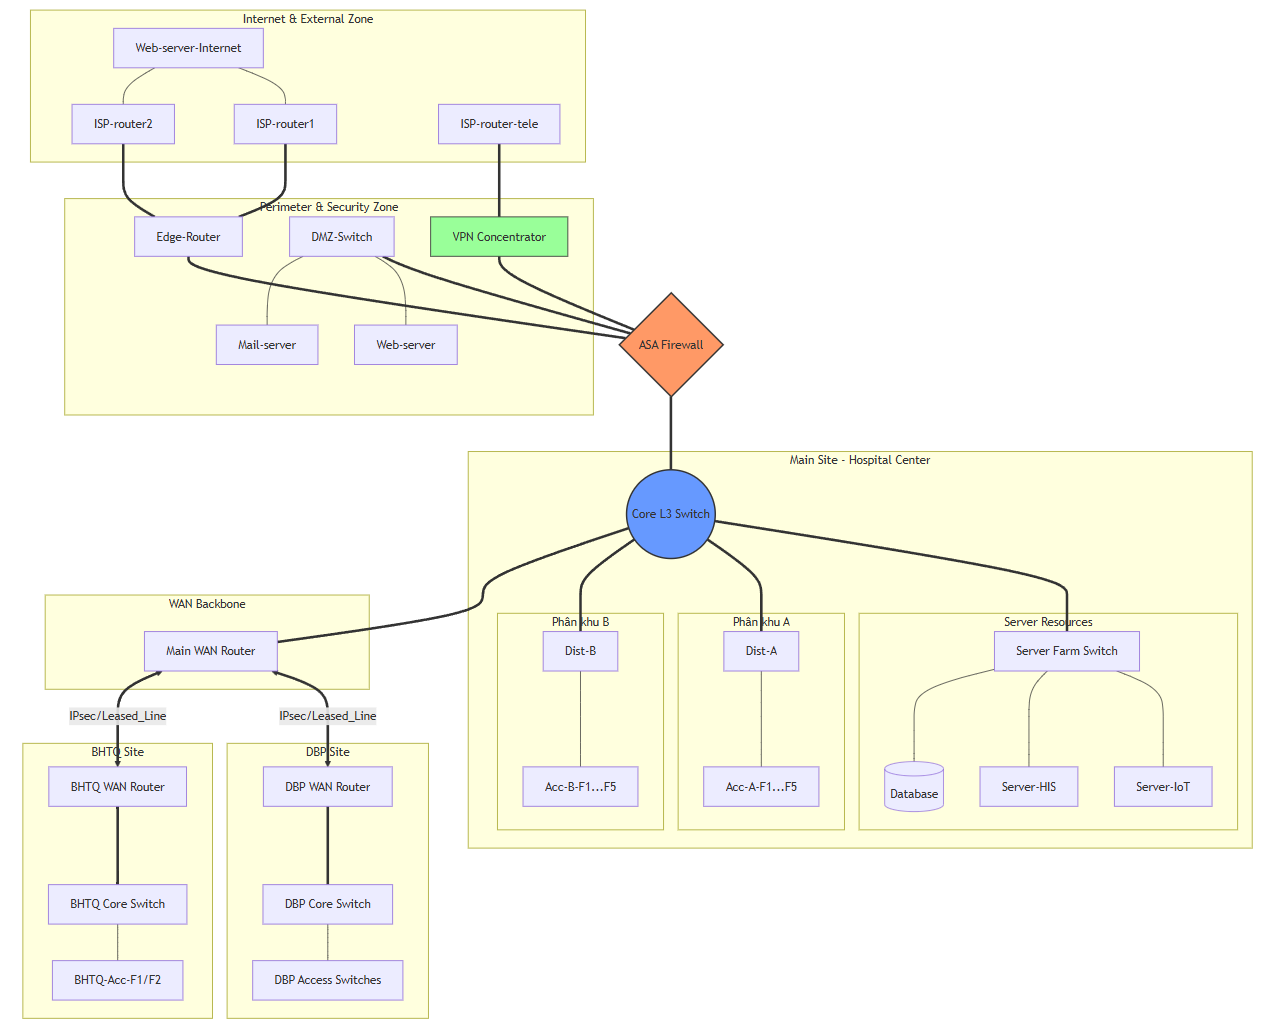
\includegraphics[width=0.9\textwidth]{Pkt_Images/Full-site-UML.png}
    
    % Tiêu đề của ảnh (giống với caption trong báo cáo mẫu)
    \caption{Sơ đồ mạng tổng thể}
    
    % Nhãn để trích dẫn ảnh trong bài (Ví dụ: "Như được thể hiện trong Hình \ref{fig:three_tier}")
    \label{fig:full_site_map}
\end{figure}

\subsection{Sơ đồ mạng tại Data center}
\begin{figure}[H]
    \centering
    % Điều chỉnh [width=0.9\textwidth] để ảnh chiếm 90% chiều rộng trang giấy
    % Thay "ten_anh_cua_ban.png" bằng tên file ảnh thực tế của bạn
    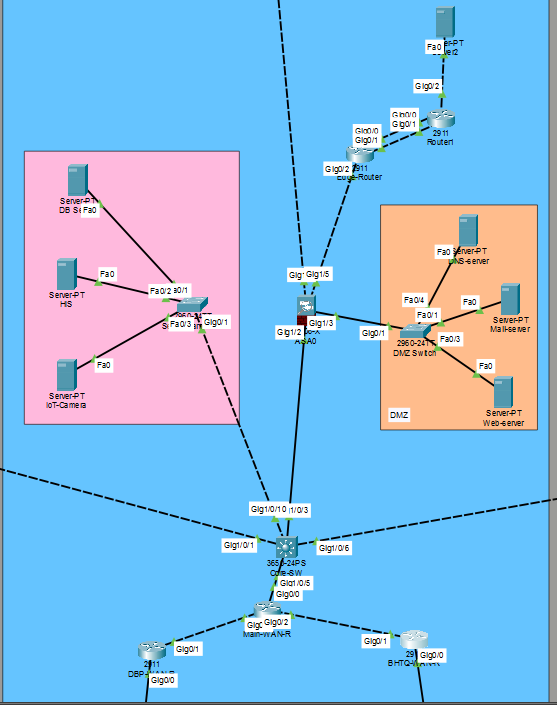
\includegraphics[width=0.4\textwidth]{Pkt_Images/Data-center.png}
    
    % Tiêu đề của ảnh (giống với caption trong báo cáo mẫu)
    \caption{Sơ đồ mạng tại Data center}
    
    % Nhãn để trích dẫn ảnh trong bài (Ví dụ: "Như được thể hiện trong Hình \ref{fig:three_tier}")
    \label{fig:data_center_map}
\end{figure}

\subsection{Sơ đồ mạng tòa A, tòa B tại trụ sở chính}
\begin{figure}[H]
    \centering
    % Hình thứ nhất (bên trái)
    \begin{subfigure}[b]{0.48\textwidth}
        \centering
        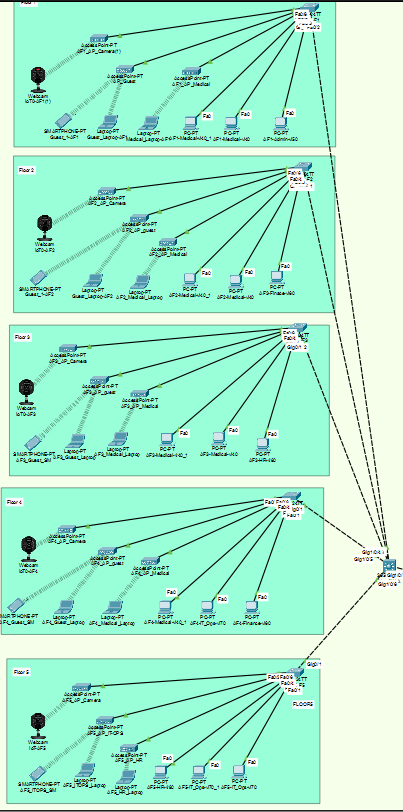
\includegraphics[width=\textwidth]{Pkt_Images/site-A.png}
        \caption{Sơ đồ mạng Tòa A}
        \label{fig:toa_a}
    \end{subfigure}
    \hfill % Tạo khoảng trống tối đa giữa 2 hình
    % Hình thứ hai (bên phải)
    \begin{subfigure}[b]{0.48\textwidth}
        \centering
        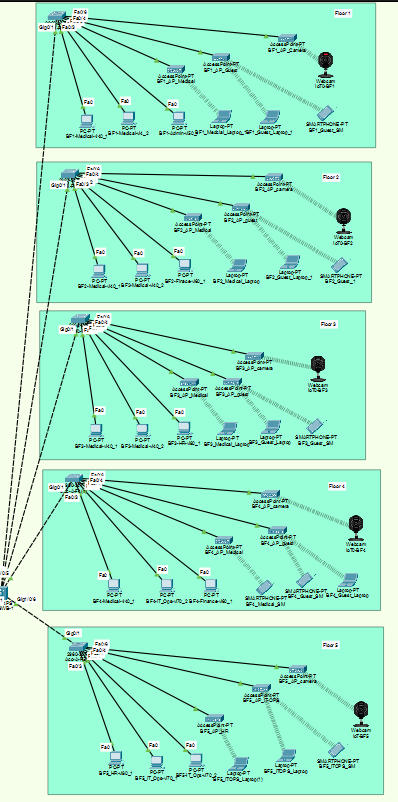
\includegraphics[width=\textwidth]{Pkt_Images/site-B.png}
        \caption{Sơ đồ mạng Tòa B}
        \label{fig:toa_b}
    \end{subfigure}

    \caption{Sơ đồ mạng tòa A và tòa B tại trụ sở chính}
    \label{fig:network_toa_ab}
\end{figure}

\subsection{Sơ đồ mạng tại trụ sở DBP và trụ sở BHTQ}
\subsubsection{Tại trụ sở DBP}
\begin{figure}[H]
    \centering
    % Điều chỉnh [width=0.9\textwidth] để ảnh chiếm 90% chiều rộng trang giấy
    % Thay "ten_anh_cua_ban.png" bằng tên file ảnh thực tế của bạn
    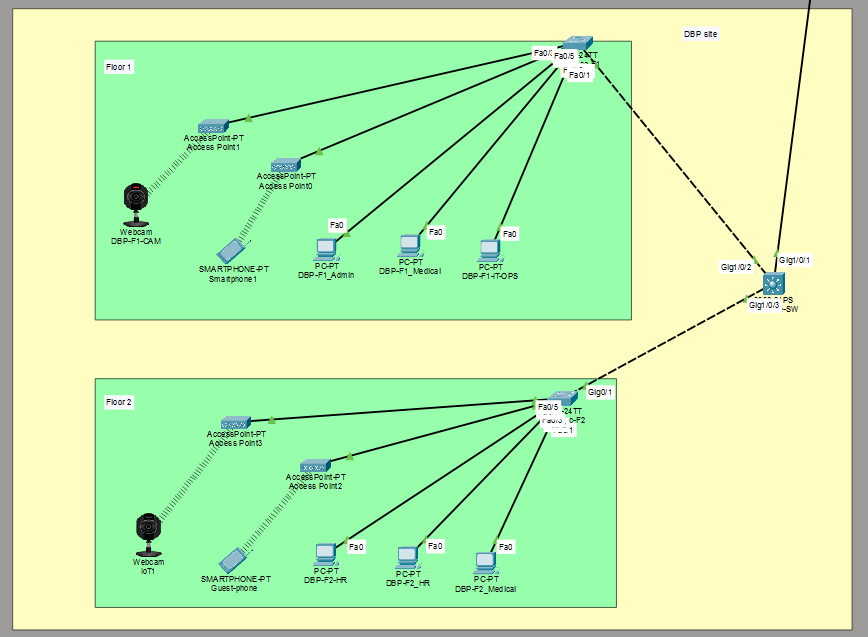
\includegraphics[width=0.6\textwidth]{Pkt_Images/DBP-site.png}
    
    % Tiêu đề của ảnh (giống với caption trong báo cáo mẫu)
    \caption{Sơ đồ mạng tại trụ sở DBP}
    
    % Nhãn để trích dẫn ảnh trong bài (Ví dụ: "Như được thể hiện trong Hình \ref{fig:three_tier}")
    \label{fig:dbp_site_map}
\end{figure}
\subsubsection{Tại trụ sở BHTQ}
\begin{figure}[H]
    \centering
    % Điều chỉnh [width=0.9\textwidth] để ảnh chiếm 90% chiều rộng trang giấy
    % Thay "ten_anh_cua_ban.png" bằng tên file ảnh thực tế của bạn
    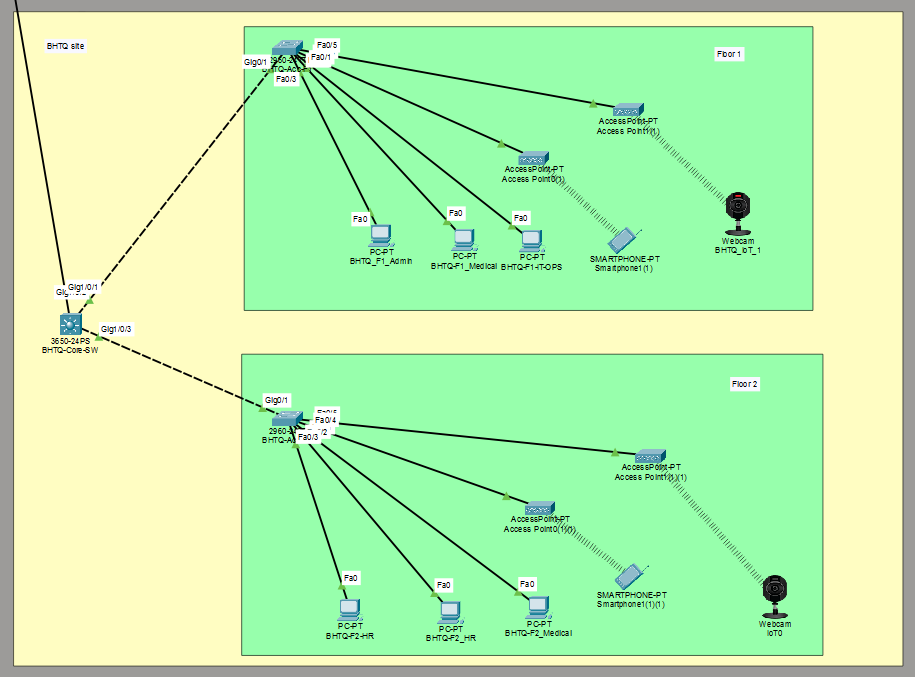
\includegraphics[width=0.6\textwidth]{Pkt_Images/BHTQ-site.png}
    
    % Tiêu đề của ảnh (giống với caption trong báo cáo mẫu)
    \caption{Sơ đồ mạng tại trụ sở BHTQ}
    
    % Nhãn để trích dẫn ảnh trong bài (Ví dụ: "Như được thể hiện trong Hình \ref{fig:three_tier}")
    \label{fig:bhtq_site_map}
\end{figure}

\subsection{Mô tả sơ bộ cho thiết kế hệ thống mạng}

\subsubsection{Phân vùng biên và Bảo mật (Edge \& Security Zone)}
Hệ thống kết nối với Internet thông qua các thiết bị sau:
\begin{itemize}
    \item \textbf{Internet \& External Zone:} Sử dụng đa kết nối ISP (2 đường truyền) để đảm bảo tính dự phòng, một đường truyền riêng (ISP-router-tele) được dành cho kết nối VPN.
    \item \textbf{ASA Firewall:} Đóng vai trò là trung tâm kiểm soát luồng dữ liệu (Hub). Mọi lưu lượng từ bên ngoài vào hệ thống nội bộ hoặc vùng DMZ đều phải đi qua kiểm tra tại đây.
    \item \textbf{Vùng DMZ:} Chứa các Server công cộng như Web-server và Mail-server, được tách biệt với mạng nội bộ qua DMZ-Switch để giảm thiểu rủi ro bị tấn công trực diện vào cơ sở dữ liệu.
    \item \textbf{VPN Concentrator:} Cho phép các kết nối từ xa truy cập an toàn vào hệ thống thông qua các đường truyền được mã hóa.
\end{itemize}

\subsubsection{Cấu trúc mạng tại Trụ sở chính (Main Site)}
Mạng nội bộ tại trụ sở chính được thiết kế theo mô hình 3 lớp tiêu chuẩn:
\begin{itemize}
    \item \textbf{Core Layer (Lớp lõi):} Sử dụng thiết bị \textbf{Core L3 Switch} hiệu năng cao, chịu trách nhiệm chuyển mạch gói tin tốc độ cao giữa các phân khu, Server Farm và kết nối WAN.
    \item \textbf{Distribution Layer (Lớp phân phối):} Gồm các Switch \textbf{Dist-A} và \textbf{Dist-B}, đóng vai trò hội tụ dữ liệu từ các tầng (F1-F5), thực hiện định tuyến và áp đặt các chính sách truy cập (ACLs).
    \item \textbf{Access Layer (Lớp truy cập):} Các Switch truy cập (Acc-A, Acc-B) kết nối trực tiếp với thiết bị đầu cuối của người dùng tại các tầng từ 1 đến 5.
\end{itemize}

\subsubsection{Trung tâm dữ liệu và Máy chủ (Server Farm)}
Các tài nguyên quan trọng được tập trung tại \textbf{Server Farm Switch}:
\begin{itemize}
    \item \textbf{Server HIS:} Hệ thống thông tin bệnh viện (Hospital Information System).
    \item \textbf{Server IoT:} Quản lý dữ liệu từ các thiết bị IoT (Camera).
    \item \textbf{Database (DB):} Hệ quản trị cơ sở dữ liệu dùng chung, được bảo vệ sâu nhất trong cấu trúc mạng.
\end{itemize}

\subsubsection{Kết nối liên chi nhánh (WAN Infrastructure)}
Hệ thống mở rộng kết nối tới các chi nhánh (DBP Site và BHTQ Site) thông qua trục \textbf{WAN Backbone}:
\begin{itemize}
    \item \textbf{Main WAN Router:} Thực hiện kết nối tới các Router chi nhánh thông qua công nghệ \textit{IPsec VPN} hoặc đường thuê riêng \textit{Leased Line}.
    \item \textbf{Tại các chi nhánh:} Sử dụng cấu trúc thu gọn (Collapsed Core) với WAN Router kết nối trực tiếp xuống Core/Dist Switch và tỏa ra các Access Switch, đảm bảo đầy đủ tính năng quản lý.
\end{itemize}



\newpage
\section{Kiểm thử hệ thống}

\subsection{Kết nối các thiết bị trong cùng VLAN}
Chọn 2 thiết bị trong cùng VLAN:
\begin{figure}[H]
    \centering
    % Điều chỉnh [width=0.9\textwidth] để ảnh chiếm 90% chiều rộng trang giấy
    % Thay "ten_anh_cua_ban.png" bằng tên file ảnh thực tế của bạn
    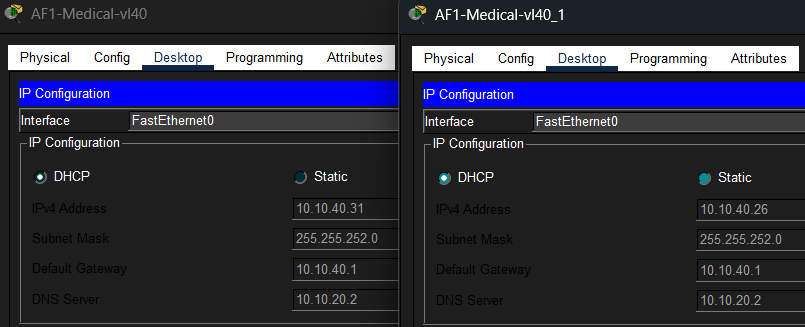
\includegraphics[width=0.8\textwidth]{Pkt_Images/1-2-ip-in-same-LAN.png}
    
    % Tiêu đề của ảnh (giống với caption trong báo cáo mẫu)
    \caption{Địa chỉ IP của 2 thiết bị trong VLAN Medical}
    
    % Nhãn để trích dẫn ảnh trong bài (Ví dụ: "Như được thể hiện trong Hình \ref{fig:three_tier}")
    \label{fig:ip_config_medical}
\end{figure}
\begin{figure}[H]
    \centering
    % Điều chỉnh [width=0.9\textwidth] để ảnh chiếm 90% chiều rộng trang giấy
    % Thay "ten_anh_cua_ban.png" bằng tên file ảnh thực tế của bạn
    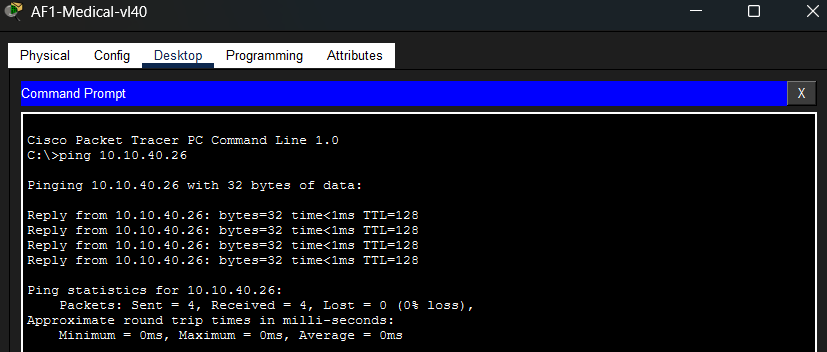
\includegraphics[width=0.8\textwidth]{Pkt_Images/1-ping-success-in-same-VLAN.png}
    
    % Tiêu đề của ảnh (giống với caption trong báo cáo mẫu)
    \caption{Kết quả ping giữa 2 thiết bị trong VLAN Medical}
    
    % Nhãn để trích dẫn ảnh trong bài (Ví dụ: "Như được thể hiện trong Hình \ref{fig:three_tier}")
    \label{fig:medical_to_medical}
\end{figure}

\subsection{Kết nối các thiết bị giữa các VLAN khác nhau}
Chọn 2 thiết bị trong các VLAN khác nhau:
\begin{figure}[H]
    \centering
    % Điều chỉnh [width=0.9\textwidth] để ảnh chiếm 90% chiều rộng trang giấy
    % Thay "ten_anh_cua_ban.png" bằng tên file ảnh thực tế của bạn
    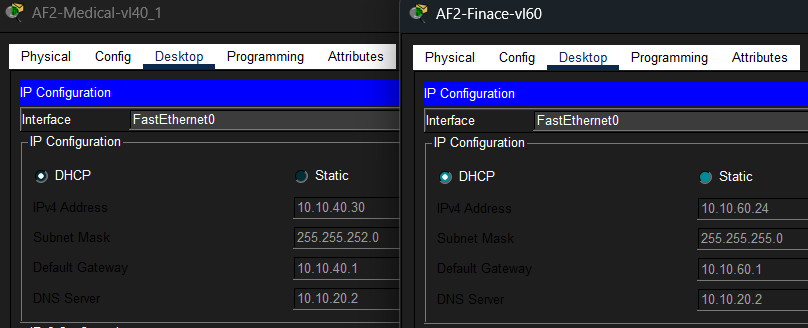
\includegraphics[width=0.8\textwidth]{Pkt_Images/2-2-ip-in-diff-VLAN.png}
    
    % Tiêu đề của ảnh (giống với caption trong báo cáo mẫu)
    \caption{Địa chỉ IP của 2 thiết bị trong VLAN FINANCE và VLAN MEDICAL}
    
    % Nhãn để trích dẫn ảnh trong bài (Ví dụ: "Như được thể hiện trong Hình \ref{fig:three_tier}")
    \label{fig:ip_config_finance}
\end{figure}
\begin{figure}[H]
    \centering
    % Điều chỉnh [width=0.9\textwidth] để ảnh chiếm 90% chiều rộng trang giấy
    % Thay "ten_anh_cua_ban.png" bằng tên file ảnh thực tế của bạn
    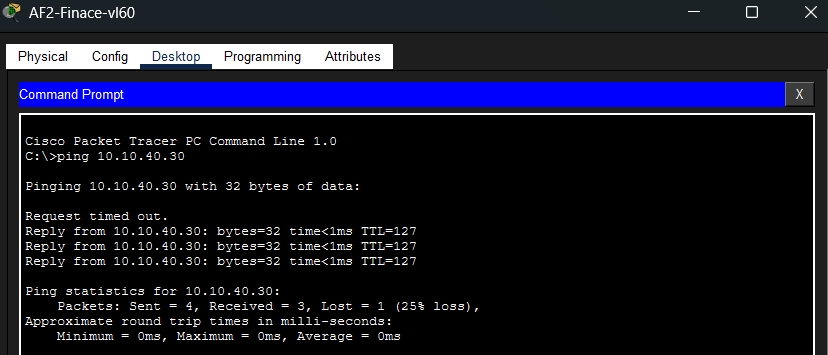
\includegraphics[width=0.8\textwidth]{Pkt_Images/2-ping-success-in-diff-VLAN.png}
    
    % Tiêu đề của ảnh (giống với caption trong báo cáo mẫu)
    \caption{Kết quả ping giữa 2 thiết bị trong VLAN FINANCE và VLAN MEDICAL}
    
    % Nhãn để trích dẫn ảnh trong bài (Ví dụ: "Như được thể hiện trong Hình \ref{fig:three_tier}")
    \label{fig:hr_to_finance}
\end{figure}
\subsection{Kết nối các thiết bị giữa trụ sở chính và hai trụ sở phụ}
\begin{figure}[H]
    \centering
    % Điều chỉnh [width=0.9\textwidth] để ảnh chiếm 90% chiều rộng trang giấy
    % Thay "ten_anh_cua_ban.png" bằng tên file ảnh thực tế của bạn
    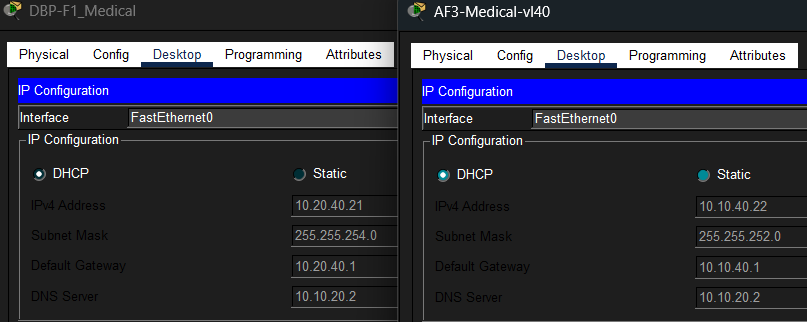
\includegraphics[width=0.8\textwidth]{Pkt_Images/3-2-ip-diff-site.png}
    
    % Tiêu đề của ảnh (giống với caption trong báo cáo mẫu)
    \caption{Địa chỉ IP của thiết bị tại trụ sở chính và thiết bị tại trụ sở DBP}
    
    % Nhãn để trích dẫn ảnh trong bài (Ví dụ: "Như được thể hiện trong Hình \ref{fig:three_tier}")
    \label{fig:ip_config_dbp_main}
\end{figure}
\begin{figure}[H]
    \centering
    % Điều chỉnh [width=0.9\textwidth] để ảnh chiếm 90% chiều rộng trang giấy
    % Thay "ten_anh_cua_ban.png" bằng tên file ảnh thực tế của bạn
    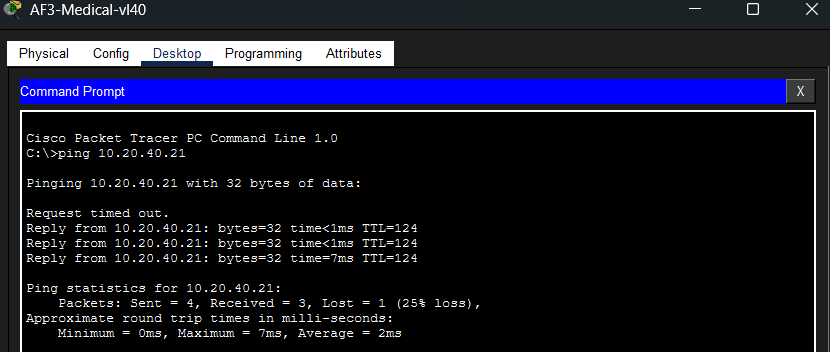
\includegraphics[width=0.8\textwidth]{Pkt_Images/3-ping-success.png}
    
    % Tiêu đề của ảnh (giống với caption trong báo cáo mẫu)
    \caption{Kết quả ping giữa thiết bị tại trụ sở chính và thiết bị tại trụ sở DBP}
    
    % Nhãn để trích dẫn ảnh trong bài (Ví dụ: "Như được thể hiện trong Hình \ref{fig:three_tier}")
    \label{fig:main_to_dbp}
\end{figure}
\subsection{Kết nối đến server DMZ}
\begin{figure}[H]
    \centering
    % Điều chỉnh [width=0.9\textwidth] để ảnh chiếm 90% chiều rộng trang giấy
    % Thay "ten_anh_cua_ban.png" bằng tên file ảnh thực tế của bạn
    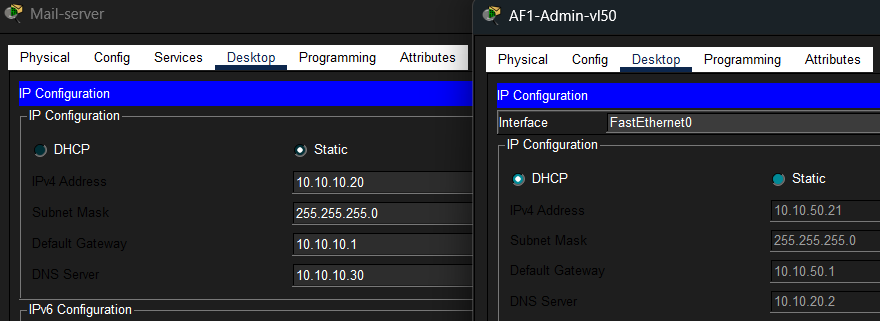
\includegraphics[width=0.8\textwidth]{Pkt_Images/4-2-ip.png}
    
    % Tiêu đề của ảnh (giống với caption trong báo cáo mẫu)
    \caption{Địa chỉ IP của Mail Server trong DMZ và đia chỉ IP của thiết bị trong VLAN ADMIN}
    
    % Nhãn để trích dẫn ảnh trong bài (Ví dụ: "Như được thể hiện trong Hình \ref{fig:three_tier}")
    \label{fig:ip_config_mailserver}
\end{figure}
\begin{figure}[H]
    \centering
    % Điều chỉnh [width=0.9\textwidth] để ảnh chiếm 90% chiều rộng trang giấy
    % Thay "ten_anh_cua_ban.png" bằng tên file ảnh thực tế của bạn
    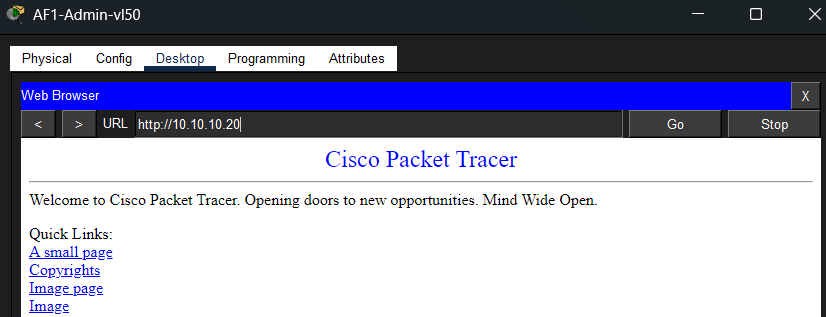
\includegraphics[width=0.8\textwidth]{Pkt_Images/4-mail-server.png}
    
    % Tiêu đề của ảnh (giống với caption trong báo cáo mẫu)
    \caption{Truy cập Mail server từ trình duyệt của thiết bị (Web Server) trong VLAN ADMIN}
    
    % Nhãn để trích dẫn ảnh trong bài (Ví dụ: "Như được thể hiện trong Hình \ref{fig:three_tier}")
    \label{fig:admin_to_mailserver}
\end{figure}
\begin{figure}[H]
    \centering
    % Điều chỉnh [width=0.9\textwidth] để ảnh chiếm 90% chiều rộng trang giấy
    % Thay "ten_anh_cua_ban.png" bằng tên file ảnh thực tế của bạn
    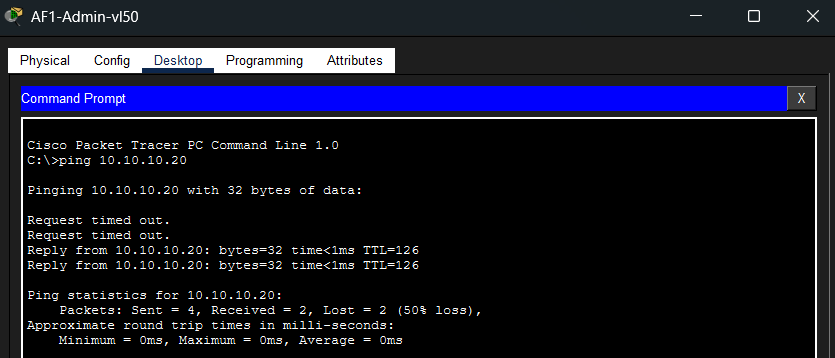
\includegraphics[width=0.8\textwidth]{Pkt_Images/4-ping-success.png}
    
    % Tiêu đề của ảnh (giống với caption trong báo cáo mẫu)
    \caption{Kết quả ping từ thiết bị trong VLAN ADMIN đến Mail Server trong DMZ}
    
    % Nhãn để trích dẫn ảnh trong bài (Ví dụ: "Như được thể hiện trong Hình \ref{fig:three_tier}")
    \label{fig:admin_to_mailserver}
\end{figure}

\subsection{Chặn truy cập từ GUEST đến các VLAN nội bộ}
\begin{figure}[H]
    \centering
    % Điều chỉnh [width=0.9\textwidth] để ảnh chiếm 90% chiều rộng trang giấy
    % Thay "ten_anh_cua_ban.png" bằng tên file ảnh thực tế của bạn
    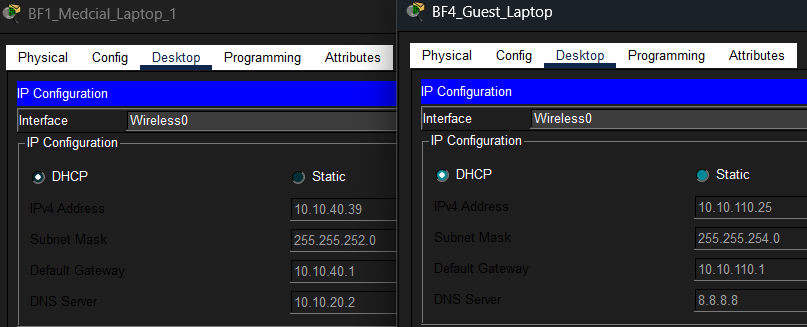
\includegraphics[width=0.8\textwidth]{Pkt_Images/5-2-ip.png}
    
    % Tiêu đề của ảnh (giống với caption trong báo cáo mẫu)
    \caption{Địa chỉ IP của thiết bị trong VLAN GUEST và thiết bị trong VLAN MEDICAL(tại trụ sở chính)}
    
    % Nhãn để trích dẫn ảnh trong bài (Ví dụ: "Như được thể hiện trong Hình \ref{fig:three_tier}")
    \label{fig:ip_config_medical_2}
\end{figure}
\begin{figure}[H]
    \centering
    % Điều chỉnh [width=0.9\textwidth] để ảnh chiếm 90% chiều rộng trang giấy
    % Thay "ten_anh_cua_ban.png" bằng tên file ảnh thực tế của bạn
    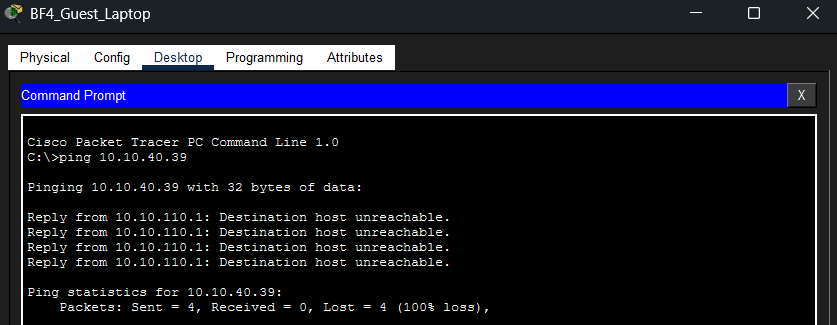
\includegraphics[width=0.8\textwidth]{Pkt_Images/5-ping-fail.png}
    
    % Tiêu đề của ảnh (giống với caption trong báo cáo mẫu)
    \caption{Kết quả ping từ thiết bị trong VLAN GUEST đến thiết bị trong VLAN MEDICAL tại trụ sở chính}
    
    % Nhãn để trích dẫn ảnh trong bài (Ví dụ: "Như được thể hiện trong Hình \ref{fig:three_tier}")
    \label{fig:guest_to_medical}
\end{figure}
\begin{figure}[H]
    \centering
    % Điều chỉnh [width=0.9\textwidth] để ảnh chiếm 90% chiều rộng trang giấy
    % Thay "ten_anh_cua_ban.png" bằng tên file ảnh thực tế của bạn
    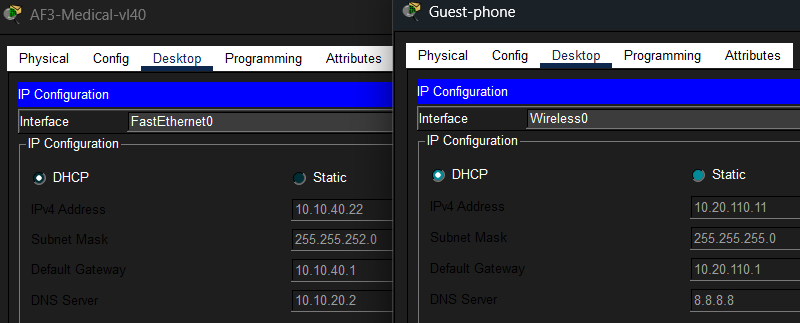
\includegraphics[width=0.8\textwidth]{Pkt_Images/5-ip-MAIN-DBP-site.png}
    
    % Tiêu đề của ảnh (giống với caption trong báo cáo mẫu)
    \caption{Địa chỉ IP của thiết bị trong VLAN GUEST(tại trụ sở DBP) và thiết bị trong VLAN MEDICAL(tại trụ sở chính)}
    
    % Nhãn để trích dẫn ảnh trong bài (Ví dụ: "Như được thể hiện trong Hình \ref{fig:three_tier}")
    \label{fig:ip_config_medical_3}
\end{figure}
\begin{figure}[H]
    \centering
    % Điều chỉnh [width=0.9\textwidth] để ảnh chiếm 90% chiều rộng trang giấy
    % Thay "ten_anh_cua_ban.png" bằng tên file ảnh thực tế của bạn
    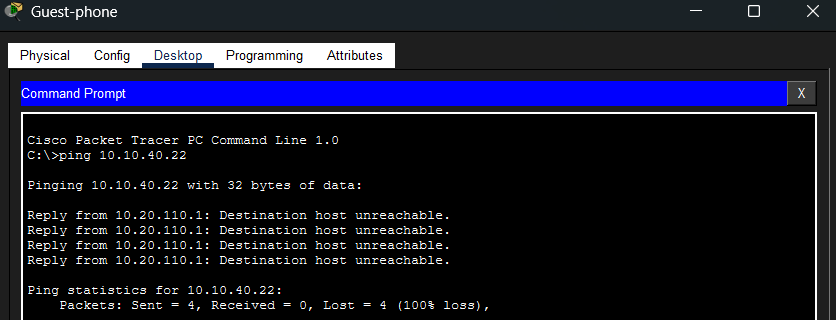
\includegraphics[width=0.8\textwidth]{Pkt_Images/5-ping-fail-DBP-site.png}
    
    % Tiêu đề của ảnh (giống với caption trong báo cáo mẫu)
    \caption{Kết quả ping từ thiết bị trong VLAN GUEST(tại trụ sở DBP) đến thiết bị trong VLAN MEDICAL (tại trụ sở chính)}
    
    % Nhãn để trích dẫn ảnh trong bài (Ví dụ: "Như được thể hiện trong Hình \ref{fig:three_tier}")
    \label{fig:guest_to_medical_1}
\end{figure}
\subsection{Kết nối Internet đến Webserver}
\textbf{Tại trụ sở chính:}
\begin{figure}[H]
    \centering
    % Điều chỉnh [width=0.9\textwidth] để ảnh chiếm 90% chiều rộng trang giấy
    % Thay "ten_anh_cua_ban.png" bằng tên file ảnh thực tế của bạn
    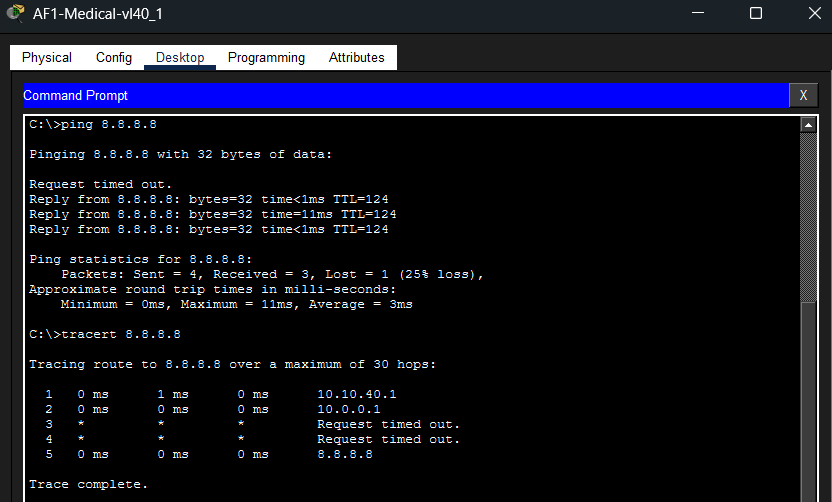
\includegraphics[width=0.8\textwidth]{Pkt_Images/6-Main-to-Internet.png}
    
    % Tiêu đề của ảnh (giống với caption trong báo cáo mẫu)
    \caption{Kết quả ping từ thiết bị trong VLAN MEDICAL (tại cơ sở chính) đến địa chỉ IP public của Internet}
    % Nhãn để trích dẫn ảnh trong bài (Ví dụ: "Như được thể hiện trong Hình \ref{fig:three_tier}")
    \label{fig:ip_main_to_internet}
\end{figure}
\begin{figure}[H]
    \centering
    % Điều chỉnh [width=0.9\textwidth] để ảnh chiếm 90% chiều rộng trang giấy
    % Thay "ten_anh_cua_ban.png" bằng tên file ảnh thực tế của bạn
    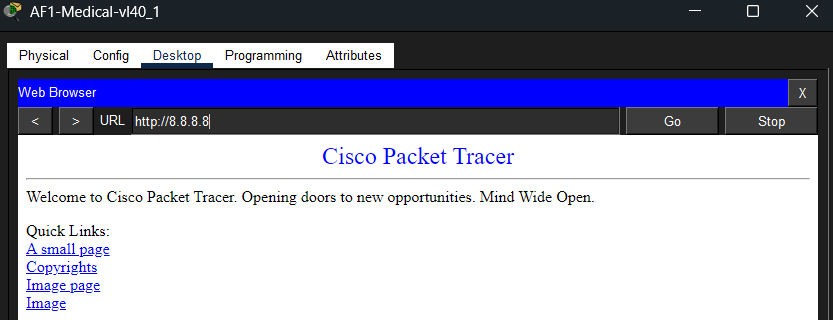
\includegraphics[width=0.8\textwidth]{Pkt_Images/6-Main-webserver.png}
    
    % Tiêu đề của ảnh (giống với caption trong báo cáo mẫu)
    \caption{Truy cập Webserver từ thiết bị trong VLAN MEDICAL qua Internet}
    
    % Nhãn để trích dẫn ảnh trong bài (Ví dụ: "Như được thể hiện trong Hình \ref{fig:three_tier}")
    \label{fig:main_to_internet_1}
\end{figure}
\textbf{Tại trụ sở BHTQ:}
\begin{figure}[H]
    \centering
    % Điều chỉnh [width=0.9\textwidth] để ảnh chiếm 90% chiều rộng trang giấy
    % Thay "ten_anh_cua_ban.png" bằng tên file ảnh thực tế của bạn
    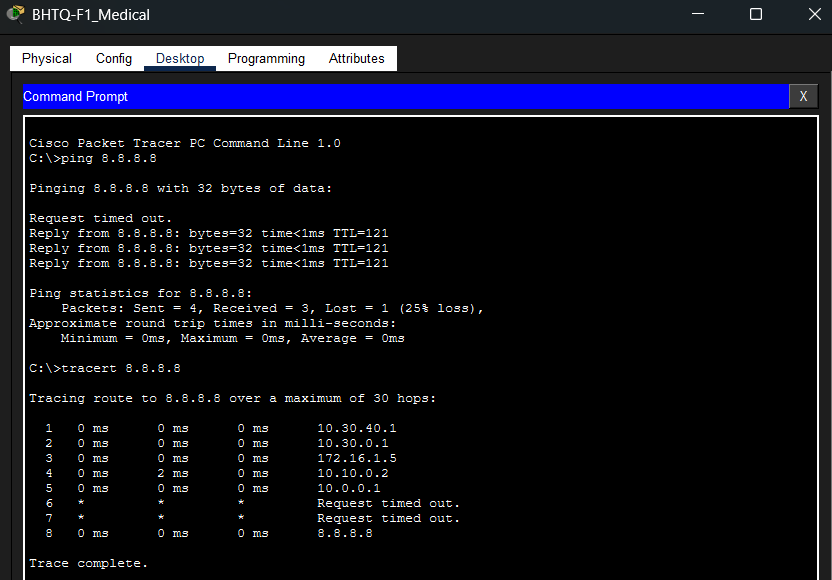
\includegraphics[width=0.8\textwidth]{Pkt_Images/6-BHTQ-to-Internet.png}
    
    % Tiêu đề của ảnh (giống với caption trong báo cáo mẫu)
    \caption{Kết quả ping từ thiết bị trong VLAN MEDICAL (tại cơ sở BHTQ) đến địa chỉ IP public của Internet}
    % Nhãn để trích dẫn ảnh trong bài (Ví dụ: "Như được thể hiện trong Hình \ref{fig:three_tier}")
    \label{fig:ip_bhtq_to_internet}
\end{figure}
\begin{figure}[H]
    \centering
    % Điều chỉnh [width=0.9\textwidth] để ảnh chiếm 90% chiều rộng trang giấy
    % Thay "ten_anh_cua_ban.png" bằng tên file ảnh thực tế của bạn
    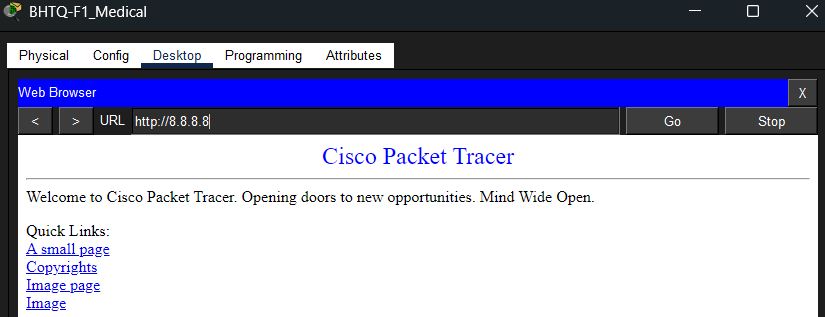
\includegraphics[width=0.8\textwidth]{Pkt_Images/6-BHTQ-webserver.png}
    
    % Tiêu đề của ảnh (giống với caption trong báo cáo mẫu)
    \caption{Truy cập Webserver từ thiết bị trong VLAN MEDICAL qua Internet}
    
    % Nhãn để trích dẫn ảnh trong bài (Ví dụ: "Như được thể hiện trong Hình \ref{fig:three_tier}")
    \label{fig:bhtq_to_internet_1}
\end{figure}

\subsection{Quản lý Camera}
\begin{figure}[H]
    \centering
    % Điều chỉnh [width=0.9\textwidth] để ảnh chiếm 90% chiều rộng trang giấy
    % Thay "ten_anh_cua_ban.png" bằng tên file ảnh thực tế của bạn
    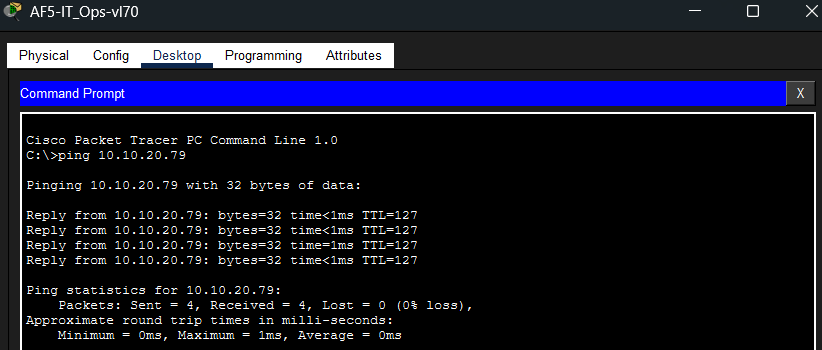
\includegraphics[width=0.8\textwidth]{Pkt_Images/7-ping-server-IoT.png}
    
    % Tiêu đề của ảnh (giống với caption trong báo cáo mẫu)
    \caption{Kết quả ping từ thiết bị trong VLAN IT-OPS đến Server IoT camera trong VLAN SERVER-FARM}
    
    % Nhãn để trích dẫn ảnh trong bài (Ví dụ: "Như được thể hiện trong Hình \ref{fig:three_tier}")
    \label{fig:ping_it_ops_to_iot}
\end{figure}
\begin{figure}[H]
    \centering
    % Điều chỉnh [width=0.9\textwidth] để ảnh chiếm 90% chiều rộng trang giấy
    % Thay "ten_anh_cua_ban.png" bằng tên file ảnh thực tế của bạn
    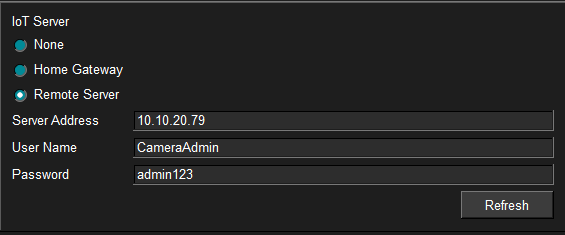
\includegraphics[width=1\textwidth]{Pkt_Images/7-username-pw.png}
    
    % Tiêu đề của ảnh (giống với caption trong báo cáo mẫu)
    \caption{Thông tin đăng nhập vào Server IoT camera}
    
    % Nhãn để trích dẫn ảnh trong bài (Ví dụ: "Như được thể hiện trong Hình \ref{fig:three_tier}")
    \label{fig:iot_username_password}
\end{figure}
\begin{figure}[H]
    \centering
    % Điều chỉnh [width=0.9\textwidth] để ảnh chiếm 90% chiều rộng trang giấy
    % Thay "ten_anh_cua_ban.png" bằng tên file ảnh thực tế của bạn
    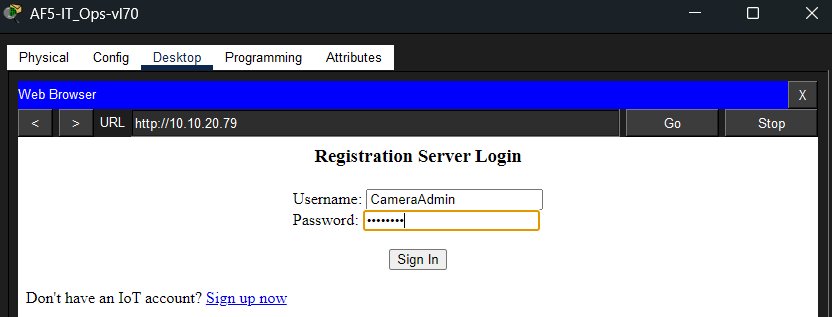
\includegraphics[width=0.8\textwidth]{Pkt_Images/7-sign-in.png}
    
    % Tiêu đề của ảnh (giống với caption trong báo cáo mẫu)
    \caption{Đăng nhập vào Server IoT camera từ thiết bị trong VLAN IT-OPS}
    
    % Nhãn để trích dẫn ảnh trong bài (Ví dụ: "Như được thể hiện trong Hình \ref{fig:three_tier}")
    \label{fig:it_ops_to_iot_1}
\end{figure}
\begin{figure}[H]
    \centering
    % Điều chỉnh [width=0.9\textwidth] để ảnh chiếm 90% chiều rộng trang giấy
    % Thay "ten_anh_cua_ban.png" bằng tên file ảnh thực tế của bạn
    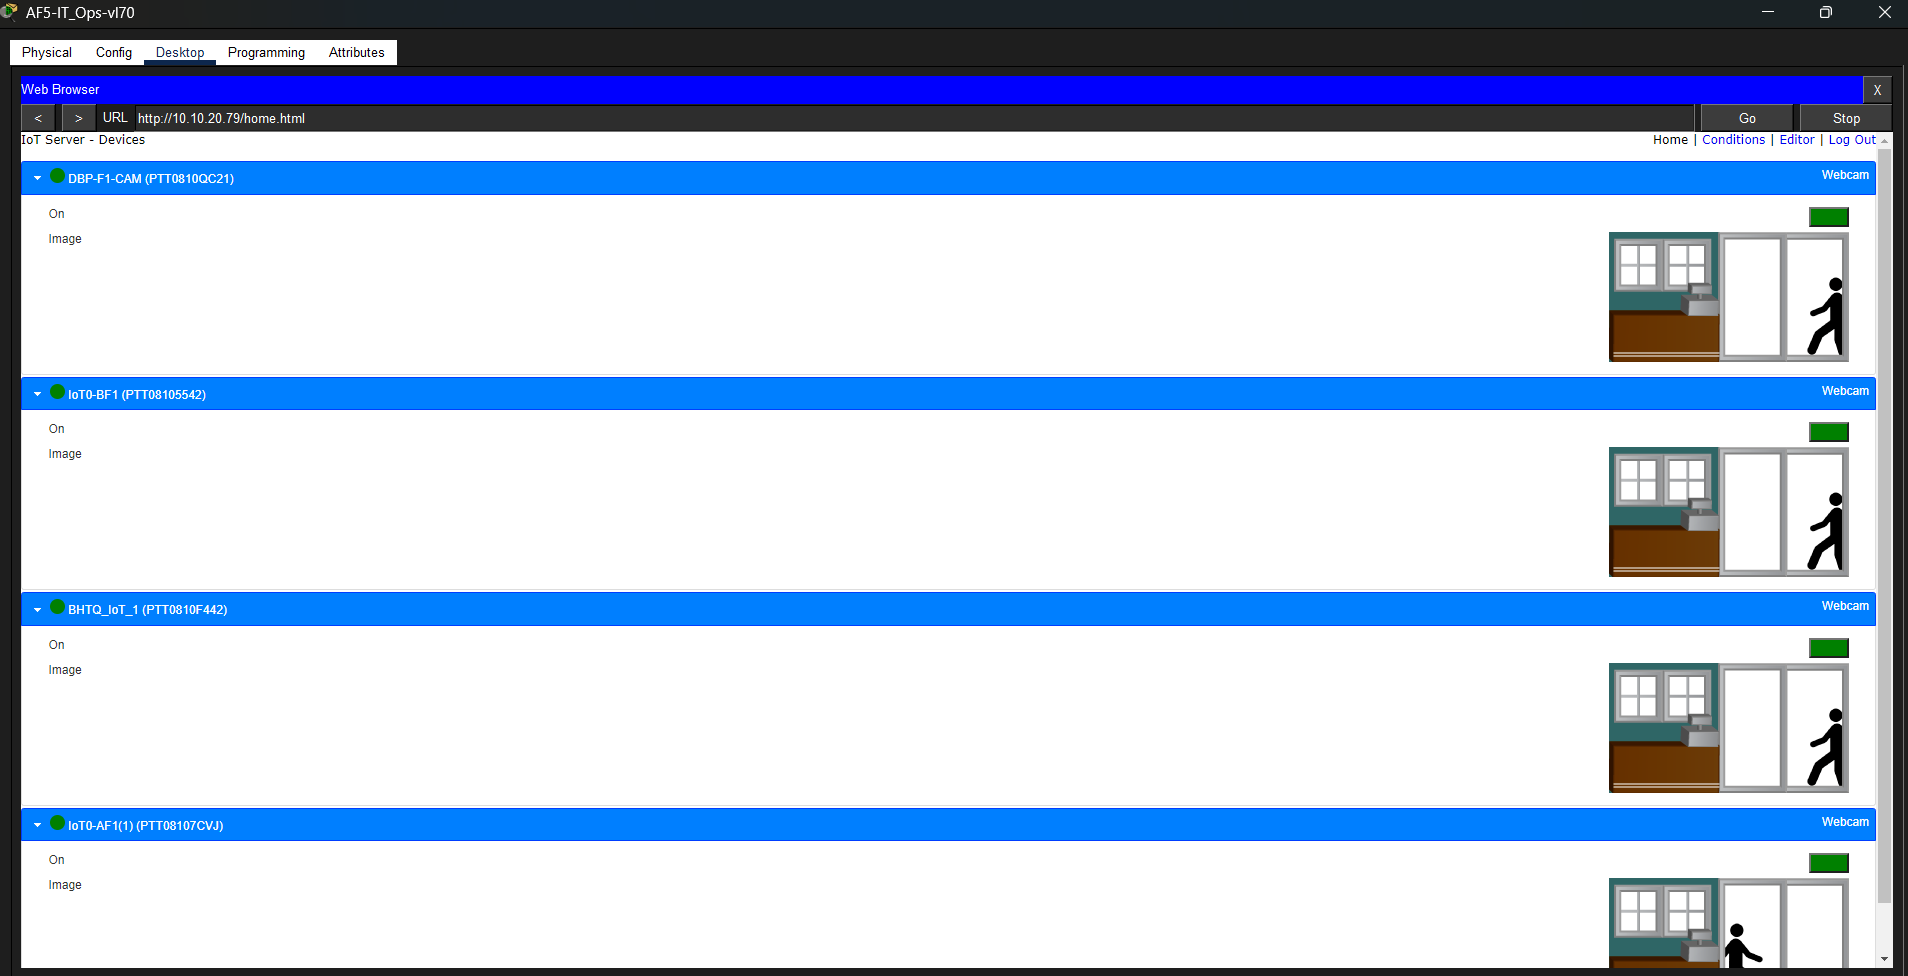
\includegraphics[width=0.8\textwidth]{Pkt_Images/7-web-server.png}
    
    % Tiêu đề của ảnh (giống với caption trong báo cáo mẫu)
    \caption{Theo dõi camera từ thiết bị trong VLAN IT-OPS}
    
    % Nhãn để trích dẫn ảnh trong bài (Ví dụ: "Như được thể hiện trong Hình \ref{fig:three_tier}")
    \label{fig:it_ops_to_iot_2}
\end{figure}
\subsection{Kết nối từ Teleworker đến các VLAN nội bộ}  
\begin{figure}[H]
    \centering
    % Điều chỉnh [width=0.9\textwidth] để ảnh chiếm 90% chiều rộng trang giấy
    % Thay "ten_anh_cua_ban.png" bằng tên file ảnh thực tế của bạn
    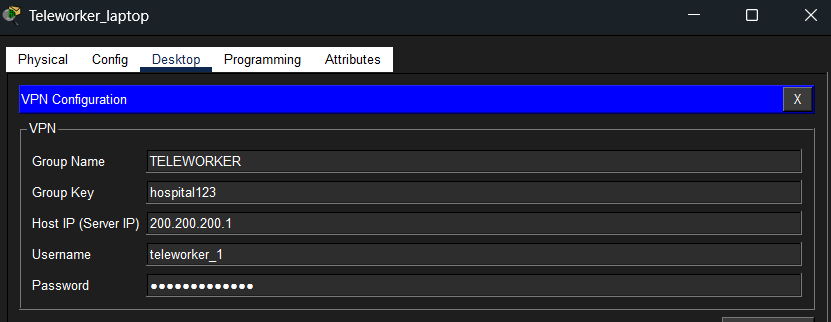
\includegraphics[width=0.8\textwidth]{Pkt_Images/8-access-VPN.png}
    
    % Tiêu đề của ảnh (giống với caption trong báo cáo mẫu)
    \caption{Thiết lập kết nối VPN từ thiết bị của Teleworker đến Firewall tại trụ sở chính}
    
    % Nhãn để trích dẫn ảnh trong bài (Ví dụ: "Như được thể hiện trong Hình \ref{fig:three_tier}")
    \label{fig:teleworker_vpn}
\end{figure}
\begin{figure}[H]
    \centering
    % Điều chỉnh [width=0.9\textwidth] để ảnh chiếm 90% chiều rộng trang giấy
    % Thay "ten_anh_cua_ban.png" bằng tên file ảnh thực tế của bạn
    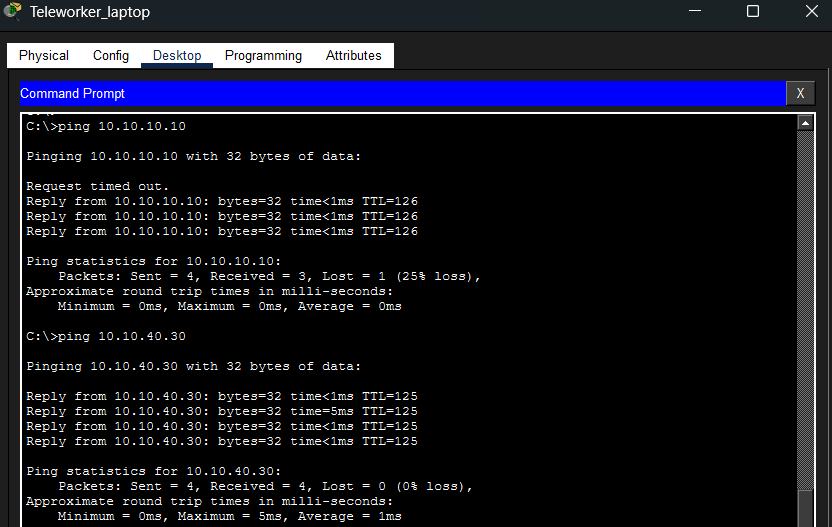
\includegraphics[width=0.8\textwidth]{Pkt_Images/8-ping-success.png}
    
    % Tiêu đề của ảnh (giống với caption trong báo cáo mẫu)
    \caption{Kết quả ping từ thiết bị của Teleworker đến thiết bị trong VLAN MEDICAL tại trụ sở chính và Webserver trong DMZ}
    
    % Nhãn để trích dẫn ảnh trong bài (Ví dụ: "Như được thể hiện trong Hình \ref{fig:three_tier}")
    \label{fig:tele_to_inter_vlan}
\end{figure}
\section{ĐÁNH GIÁ HỆ THỐNG}

\subsection{Độ tin cậy}
Hệ thống mạng được triển khai theo mô hình hình sao (Star Topology), tập trung định tuyến vào một số thiết bị chuyển mạch cốt lõi. Mặc dù dễ quản lý, thiết kế này lại tạo ra các điểm lỗi đơn lẻ (Single Point of Failure); nếu một thiết bị trung tâm gặp sự cố, toàn bộ phân đoạn mạng phía sau sẽ bị gián đoạn. Hiện tại, hệ thống định tuyến VLAN vẫn phụ thuộc nhiều vào cấu hình one-armed router, chưa có giải pháp sao lưu gói tin, chưa dự phòng đường truyền vật lý, và thiếu cơ chế sẵn sàng cao (High Availability - HA).

\subsection{Khả năng nâng cấp}
Một số thiết bị phần cứng trong mô hình thuộc dòng Cisco cũ (legacy), không còn được nhà sản xuất hỗ trợ cập nhật firmware hoặc các bản vá bảo mật. Điều này gây trở ngại lớn cho việc mở rộng và tích hợp các công nghệ mạng tiên tiến như IPv6, SD-WAN, hay cân bằng tải đa tuyến. Để đảm bảo khả năng nâng cấp dài hạn, hệ thống cần có lộ trình thay thế bằng các thiết bị hỗ trợ chuẩn 10GbE/40GbE và có khả năng quản trị tập trung qua giao diện Web hoặc giao thức SNMPv3.

\subsection{Phần mềm và Công cụ hỗ trợ}
Việc vận hành mạng hiện tại chủ yếu phụ thuộc vào các công cụ quản lý cục bộ tích hợp sẵn trên thiết bị. Việc chưa triển khai đồng bộ các giải pháp giám sát mạng chuyên nghiệp (như Zabbix, PRTG, hay SolarWinds) làm hạn chế khả năng thống kê, phân tích hiệu năng và cảnh báo sự cố theo thời gian thực. Hơn nữa, các thao tác bảo trì, cấu hình và sao lưu vẫn phải thực hiện hoàn toàn thủ công do thiếu vắng các công cụ tự động hóa.

\subsection{An toàn và bảo mật mạng}
Hệ thống hiện chỉ thiết lập vùng DMZ tại Trụ sở chính (Main Site), trong khi các chi nhánh đặt máy chủ nội bộ phía sau tường lửa, điều này làm giảm tính linh hoạt nếu muốn chia sẻ tải công việc trực tiếp giữa các cơ sở. Dù vậy, tường lửa ASA vẫn đang hoạt động tốt và tuân thủ đúng chính sách bảo mật cơ bản: cho phép các thiết bị nội bộ ping ra Internet nhưng chặn hoàn toàn các kết nối xâm nhập trái phép từ bên ngoài (bao gồm cả truy cập của teleworker). Tuy nhiên, để đạt độ an toàn tối đa, hệ thống cần được bổ sung các cơ chế bảo mật chiều sâu như Next-Generation Firewall hay IDS/IPS.

\subsection{Các vấn đề còn tồn tại}
Nhìn chung, cấu trúc mạng hiện tại đang đối mặt với hai vấn đề chính cần khắc phục:
\begin{itemize}
    \item Hệ thống chưa có cơ chế chuyển đổi dự phòng (Failover) tự động để đảm bảo kết nối liên tục khi thiết bị phần cứng xảy ra sự cố.
    \item Thiếu một nền tảng giám sát mạng tập trung (Network Monitoring System) để bao quát toàn bộ hạ tầng cơ sở vật chất.
\end{itemize}

\subsection{Định hướng phát triển trong tương lai}
Để đáp ứng tốc độ số hóa và quy mô của bệnh viện, trong giai đoạn tiếp theo, hệ thống cần được nâng cấp toàn diện theo các hướng sau:
\begin{itemize}
    \item \textbf{Tối ưu hóa đường truyền:} Triển khai công nghệ SD-WAN để quản lý linh hoạt và định tuyến thông minh lưu lượng giữa các chi nhánh.
    \item \textbf{Tính sẵn sàng cao:} Xây dựng cấu hình High Availability (HA) và cân bằng tải (Load Balancing) cho các thiết bị trọng yếu.
    \item \textbf{Giám sát chủ động:} Áp dụng các phần mềm giám sát mạng tập trung (Zabbix, PRTG) nhằm phát hiện và xử lý sự cố trước khi chúng ảnh hưởng đến người dùng.
    \item \textbf{Nâng cấp phần cứng:} Loại bỏ dần các thiết bị lỗi thời, chuyển sang hạ tầng hỗ trợ toàn diện IPv6, QoS nâng cao và công nghệ Clustering.
    \item \textbf{Tăng cường bảo mật:} Củng cố lớp phòng thủ bằng Next-Generation Firewall, hệ thống phát hiện/ngăn chặn xâm nhập (IDS/IPS) và thiết lập mạng riêng ảo VPN Site-to-Site đồng bộ.
\end{itemize}
\end{document}